\pdfminorversion=4
\documentclass[compress,10pt]{beamer}
%For no animations, add handout to [] options
%For no figures or top banner, add draft to [] options
%apsectratio=169 (16:9) or 54 (5:4) or 43 (4:3) or 32 (3:2)

%Load the myriad packages
\usepackage{color}
\usepackage{amssymb,amsmath}
\usepackage{textcomp}
\usepackage{graphicx}
\usepackage{tikz}
%\usepackage[numbers, super]{natbib}
\usepackage{grffile} %spaces in file names
\usepackage{parskip}
%\usepackage[T1]{fontenc} %for sc and bf
%\usepackage{times}
\usepackage{wasysym}
\usepackage{bigstrut}
\usepackage{epstopdf}
%\usepackage[dvipsnames]{xcolor}
%\usepackage{enumitem}
%\setlist{nolistsep} % or \setlist{noitemsep} to leave space around whole list
% Load some optional sub-parts of PGF
%\usetikzlibrary{decorations.pathmorphing}
%\usetikzlibrary{positioning}
%\usetikzlibrary{calc}
%\usetikzlibrary{shapes.geometric}
%\usepackage{pgfplots}
%\usepackage{rotating}
%\usepackage[no-math]{fontspec}
%\usepackage{xltxtra}
%\usepackage{xunicode}
%\defaultfontfeatures{Mapping=tex-text}
%%\setsansfont[Mapping=tex-text]{Optima}
%\setsansfont[Mapping=tex-text]{Helvetica Neue}
% Optional for code samples
%
%singular
\newcommand{\fref}[1]{Fig.~\ref{fig:#1}}
\newcommand{\Fref}[1]{Figure~\ref{fig:#1}}
\newcommand{\eref}[1]{Eq.~(\ref{eq:#1})}
\newcommand{\Eref}[1]{Equation~(\ref{eq:#1})}
\newcommand{\tref}[1]{Table~\ref{tab:#1}}
%plural
\newcommand{\frefs}[2]{Figs.~\ref{fig:#1} and \ref{fig:#2}}
\newcommand{\Frefs}[2]{Figures~\ref{fig:#1} and \ref{fig:#2}}
\newcommand{\erefs}[2]{Eqs.~(\ref{eq:#1}) and (\ref{eq:#2})}
\newcommand{\Erefs}[2]{Equations~(\ref{eq:#1}) and (\ref{eq:#2})}
\newcommand{\trefs}[2]{Tables~\ref{tab:#1} and \ref{tab:#2}}
%range
\newcommand{\frefss}[2]{Figs.~\ref{fig:#1} - \ref{fig:#2}}
\newcommand{\Frefss}[2]{Figures~\ref{fig:#1} - \ref{fig:#2}}
\newcommand{\erefss}[2]{Eqs.~(\ref{eq:#1}) - (\ref{eq:#2})}
\newcommand{\Erefss}[2]{Equations~(\ref{eq:#1}) - (\ref{eq:#2})}
\newcommand{\trefss}[2]{Tables~\ref{tab:#1} - \ref{tab:#2}}
%misc.
\newcommand{\nn}[1]{\ensuremath{^{#1}}} %[1] is # of commands
\newcommand{\keff}{\ensuremath{{k_\mathrm{eff}}}}
\newcommand{\kinf}{\ensuremath{{k_\infty}}}
\newcommand{\alphaT}{\ensuremath{{\alpha_{_T}}}}
\newcommand{\SN}{\ensuremath{{\text{S}_\text{N}}}}
\newcommand{\order}[1]{\ensuremath{\mathcal{O}\left(#1\right)}}
%Note: tarticle has ``several'' changes from article
%in this vein.
% some simplifying commands
\newcommand{\eg}{{\it e.g.}}
\newcommand{\ie}{{\it i.e.}}
\newcommand{\etal}{{\it et al.}}
\newcommand{\acite}[1]{{\bf(Add Citation: #1)}}
\newcommand{\E}{\mathcal{E}}
% derivative - d
\newcommand{\ud}{\,\mathrm{d}}
% bold unit vector n-hat
\newcommand{\nhat}{\hat{\bf n}}
\newcommand{\tensor}[1]{\mathcal{#1}}
\renewcommand{\vec}[1]{\mathbf{#1}}
\newcommand{\om}{\boldsymbol{\Omega}}

\newcommand{\tcr}[1]{\textcolor{red}{#1}}
\newcommand{\tcb}[1]{\textcolor{blue}{#1}}
\newcommand{\tcm}[1]{\textcolor{magenta}{#1}}
%

%Don't number backup slides
\newcommand{\backupbegin}{
    \newcounter{finalframe}
    \setcounter{finalframe}{\value{framenumber}}
}
\newcommand{\backupend}{
    \setcounter{framenumber}{\value{finalframe}}
}

%Colors!
\definecolor{maroon}{rgb}{0.5,0,0}
\definecolor{darkgreen}{rgb}{0,0.5,0}
\definecolor{amber}{rgb}{1.0, 0.49, 0.0}

%Get rid of navigation icons
\setbeamertemplate{navigation symbols}{}
\useoutertheme{infolines}

\setbeamercovered{transparent}
\usepackage{lipsum}

%Aggie-themed
\pgfdeclareimage[height=0.1in]{TAMUlogo}{images/tamu_engineering.png}
\pgfdeclareimage[height=0.15in]{DOElogo}{images/DOE_logo.png}
\logo{\raisebox{-8pt}{\pgfuseimage{TAMUlogo} \hspace{1pt} \pgfuseimage{DOElogo}}}
\titlegraphic{
\includegraphics[height=0.15\textheight]{images/seal.png}}

%%%%%%%%%%%%%%%%%%%%%%%%%%%%%%%%%%%%%%%%%%%%%%%%%%%%%%%%%%%%%%%
% Optional packages, used to show off certain tricks

\newlength \figwidth
\setlength \figwidth {0.5\textwidth}

\setlength{\leftmargin}{-2cm}
\setlength{\rightmargin}{-2cm}

%%%%%%%%%%%%%%%%%%%%%%%%%%%%%%%%%%%%%%%%%%%%%%%%%%%%%%%%%%%%%%%

\mode<presentation>
{
    \usepackage[english]{babel}
    \usetheme{Frankfurt}

    %Make it Aggie Maroon
    \usecolortheme[RGB={80,0,0}]{structure}

    % This will typeset only the frames (or slides) that have the given label ("current" in this case).
    %  \includeonlyframes{current}
}

\title[Polytope DGFEM Transport]{Higher-Order DGFEM Transport Calculations on Polytope Meshes for Massively-Parallel Architectures}

\author[Hackemack]{{\Large Michael W. Hackemack} \vspace{0.35cm} \\ Chair: {\small Jean C. Ragusa} \\ Committee Members: {\small Marvin L. Adams, Jim E. Morel, Nancy M. Amato } \\ External Advisor: {\small Troy Becker}}

%TAMU
\institute[Texas A\&M University]{\scriptsize Department of Nuclear Engineering\\
Texas A\&M University \\
College Station, TX, USA 77843\\[1ex]
\href{mailto:mike\_hack@tamu.edu}{mike\_hack@tamu.edu}}

\date[May 06, 2016]

% You can override the default acknowledgment, and address if you want
%\acknowledgement{*Submitted in partial fulfillment of the requirements of NUEN 610 \\
%(Nuclear Reactor Design)}
%\address{Nuclear Engineering Department \\
%            Texas A\&M University \\
%            College Station, TX 77843-3133}}

% If you don't want the menu section outline above the title, do this:
%\setbeamertemplate{headline}{}

\renewcommand{\ss}{ss}
\vfuzz=2pt

%%%%%%%%%%%%%%%%%%%%%%%%%%%%%%%%%%%%%%%%%%%%%%%%%%%%%%%%%%%%%%%%%%%%%%%%%%%%%%%%%%%%%%%%%%%%%
\begin{document}

%%%%%%%%%%%%%%%%%%%%%%%%%%%%%%%%%%%%%%%%%%%%%%%%%%%%%%%%%%%%%%%%%%%%%%%%%%%%%%%%%%%%%%%%%%%%%
%  All this typeout stuff simply gets printed to the screen as the document
% is compiled.  It helps get stuff working
\typeout{***********************************************************************************}
\typeout{titlepage}

\begin{frame}[label=title,plain]
    \titlepage
\end{frame}

%%%%%%%%%%%%%%%%%%%%%%%%%%%%%%%%%%%%%%%%%%%%%%%%%%%%%%%%%%%%%%%%%%%%%%%%%%%%%%%%%%%%%%%%%%%%%%
% TABLE OF CONTENTS
\typeout{***********************************************************************************}
\typeout{TOC}

\begin{frame}[shrink,label=toc,plain]%[plain]
    \frametitle{Outline}
    \vspace{1.1mm}
    \tableofcontents
\end{frame}

%%%%%%%%%%%%%%%%%%%%%%%%%%%%%%%%%%%%%%%%%%%%%%%%%%%%%%%%%%%%%%%%%%%%%%%%%%%%%%%%%%%%%%%%%%%%%%
\typeout{***********************************************************************************}
\typeout{Motivation}
%%%%%%%%%%%%%%%%%%%%%%%%%%%%%%%%%%%%%%%%%%%%%%%%%%%%%%%%%%%%%%%%%%%%%%%%%%%%%%%%%%%%%%%%%%%%%%
% MOTIVATION AND INTRODUCTION SECTION
\section{Motivation}
\subsection{}
% --------------------------------------------
\begin{frame}[t]\frametitle{Higher-Fidelity Transport Solutions}

\end{frame}
% --------------------------------------------
\begin{frame}[t]\frametitle{Topics of this Dissertation Work}

\end{frame}
% --------------------------------------------
\begin{frame}[t]\frametitle{The Continuous-Energy Transport Equation} \vspace{-2.5mm}
\begin{block}{Transport Equation}{\footnotesize
\begin{equation*}
\left[ { \bf \Omega} \cdot {\bf \nabla}  + \sigma_t ({\bf r}, E) \right] \psi ({\bf r}, E, {\bf \Omega}) = \int\displaylimits_{4 \pi} \int\displaylimits_{0}^{\infty}  \, \sigma_s ({\bf r}, E' , E, {\bf \Omega}' , {\bf \Omega}) \psi ({\bf r}, E', {\bf \Omega}') d E'  d \Omega'+ Q ({\bf r}, E, {\bf \Omega})
\end{equation*}
}\end{block} \vspace{-1.0mm}
\begin{block}{Boundary Conditions}{\footnotesize
\begin{equation*}
\psi ({\bf r}, E, {\bf \Omega}) = \psi^{inc} ({\bf r}, E, {\bf \Omega}) +  \int\displaylimits_{\vec{\Omega}' \cdot \vec{n} < 0} \int\displaylimits_{0}^{\infty} \beta ({\bf r}, E' , E, {\bf \Omega}' , {\bf \Omega}) \psi ({\bf r}, E', {\bf \Omega}') d E'  d \Omega'
\end{equation*}
}\end{block} \vspace{-1.0mm}
\begin{block}{Term Definitions} {\footnotesize
${\bf r}$ -  neutron position \\
$E$ -  neutron energy \\
${\bf \Omega}$ - neutron solid angle \\
$\psi  ({\bf r}, E, {\bf \Omega})$ - angular flux  \\
$Q  ({\bf r}, E, {\bf \Omega})$ - distributed neutron source \\
$\sigma_t ({\bf r}, E)$ - total macroscopic cross section \\
$\sigma_s ({\bf r}, E' , E, {\bf \Omega}' , {\bf \Omega})$ - total macroscopic scattering cross section\\
$\beta ({\bf r}, E' , E, {\bf \Omega}' , {\bf \Omega})$ - boundary albedo 
}\end{block}
\end{frame}
% --------------------------------------------
\begin{frame}[t]\frametitle{Multigroup DGFEM $S_N$ Transport Equation}

\end{frame}
% --------------------------------------------
\begin{frame}[t]\frametitle{Polytope Meshes}
         \begin{block}{}{\footnotesize
			\begin{itemize}
				\item <1-> Other physics communities are now employing polytope grids due to decreased cell/face counts (CFD in particular)
				\item <2-> They allow for transition elements between different domain regions
				\item <3-> Hanging nodes from non-conforming meshes are not necessary
				\item <4-> Independently-generated simplicial grids ({\em i.e.} created in parallel) can be stitched together with polytopes without communicating the whole mesh across processors
			\end{itemize}}
         \end{block}
\centering
\only<1>{
\vspace{0.5cm}
{}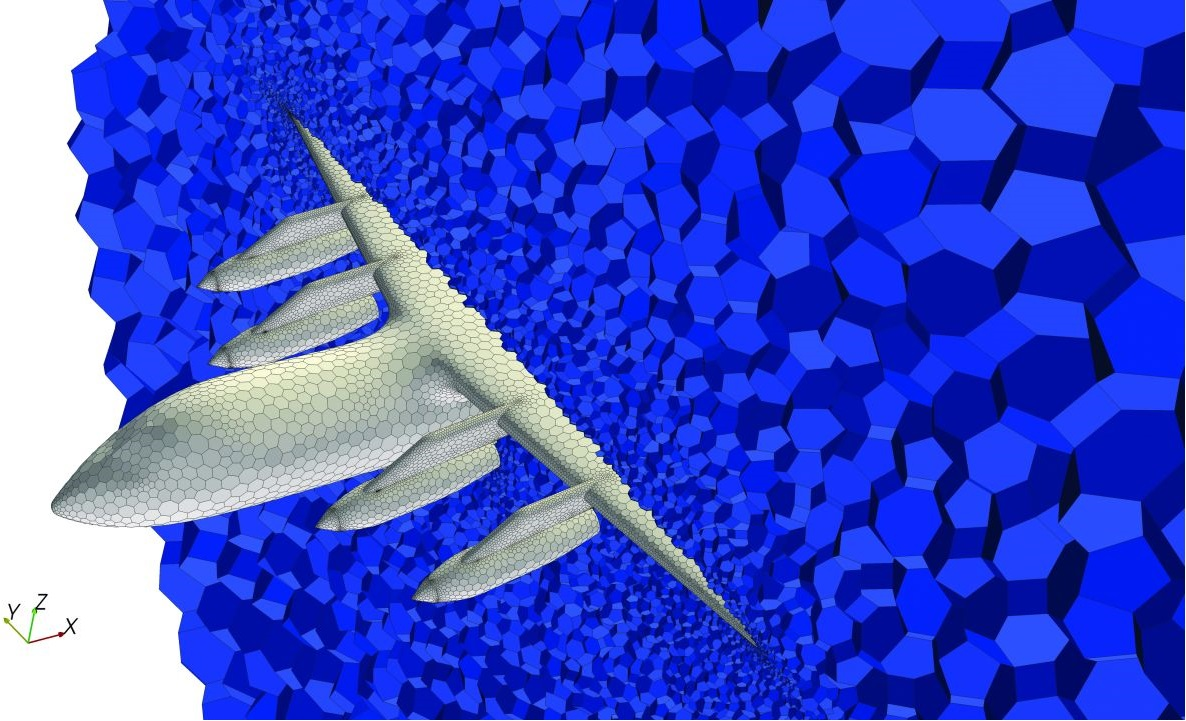
\includegraphics[width=0.45\columnwidth]{images/Polymesh_sized.jpg}
}
\only<2>{
\vspace{0.4cm}
{}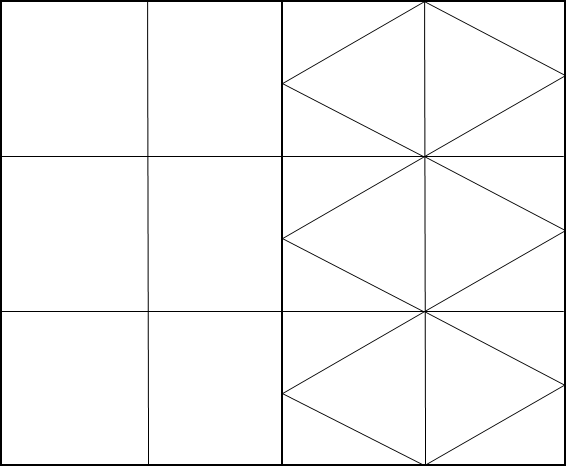
\includegraphics[width=0.4\columnwidth]{images/transition_elements_rev1.png}
}
\only<3>{
\vspace{0.5cm}
{}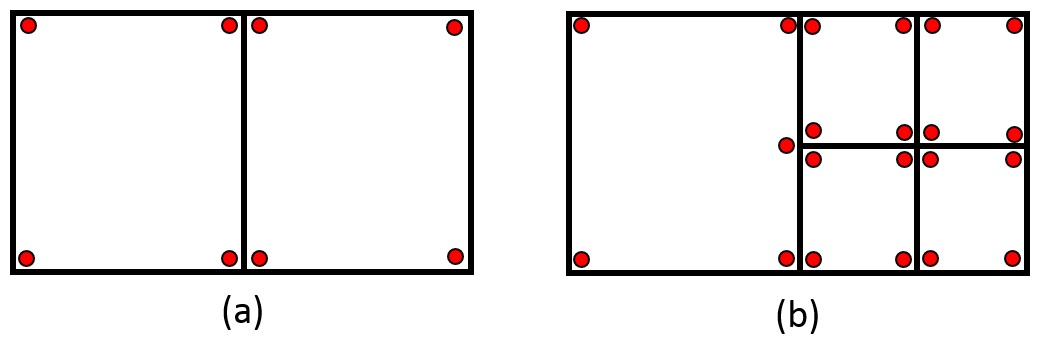
\includegraphics[width=0.65\columnwidth]{images/locally_refined_nodes.png}
}
\only<4>{
\centering
{}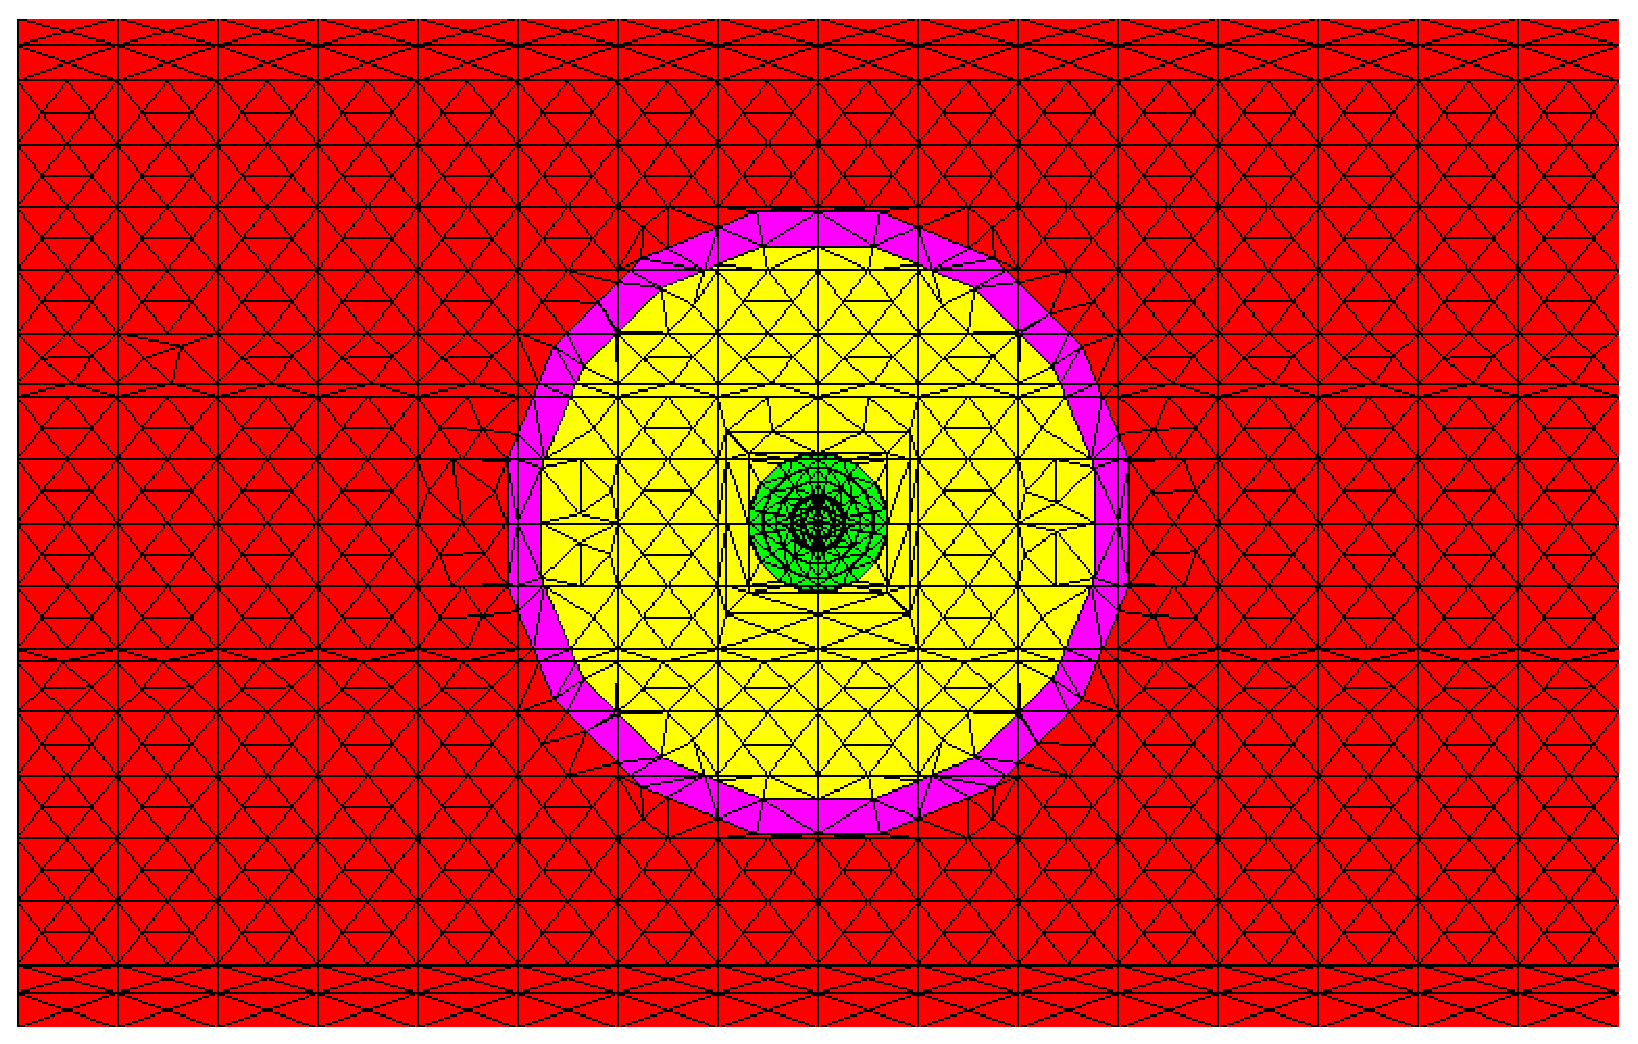
\includegraphics[width=0.52\columnwidth]{images/IM1_30_rot.eps} \hspace{1.0cm}
{}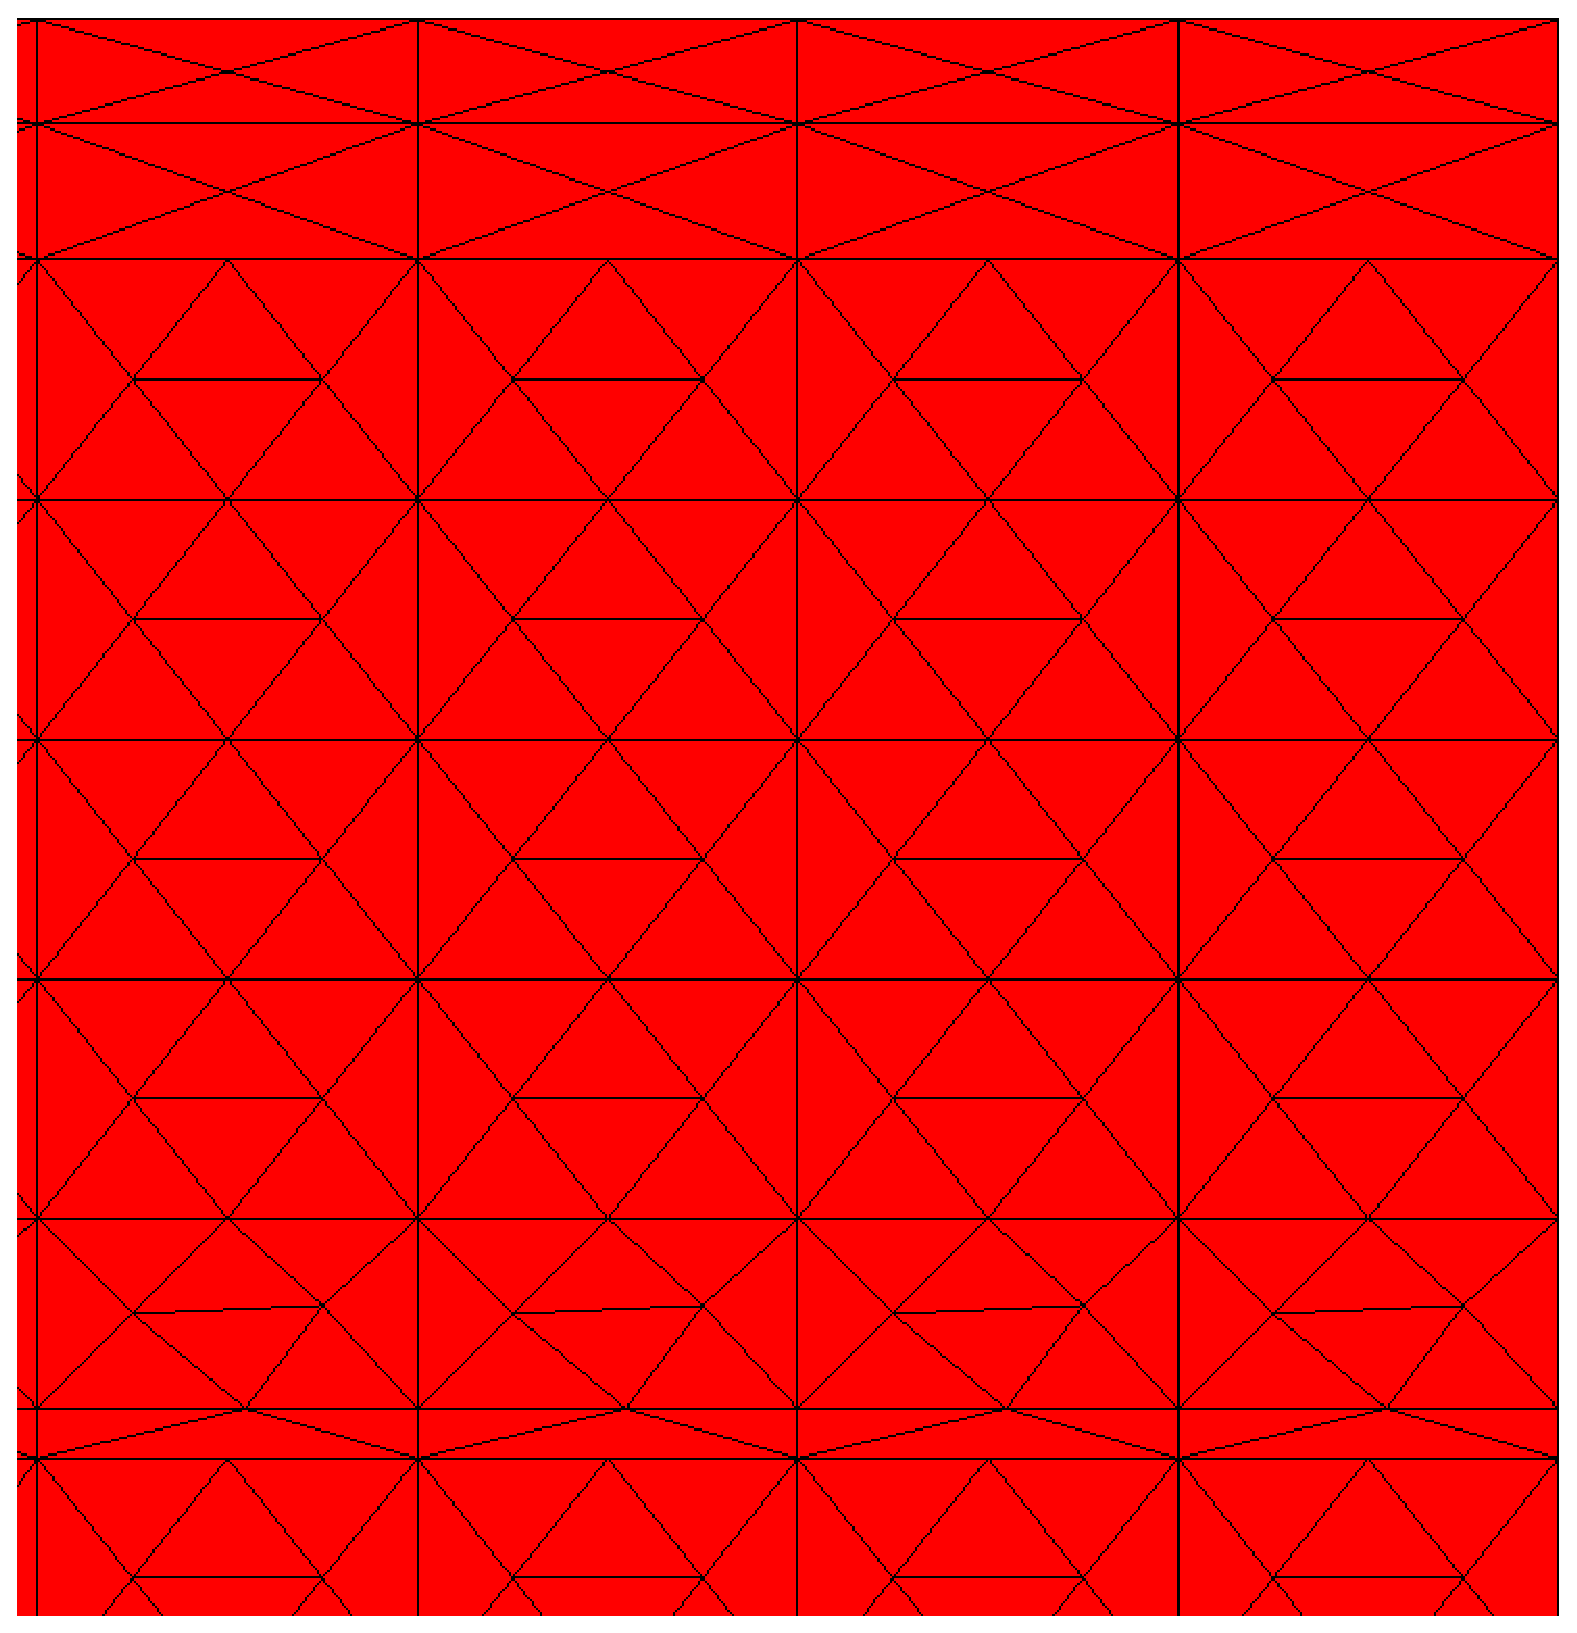
\includegraphics[width=0.345\columnwidth]{images/IM1_zoom.eps}
}
\end{frame}
% --------------------------------------------
\begin{frame}[t]\frametitle{Higher-Order FEM Basis functions}

\end{frame}
% --------------------------------------------
\begin{frame}[t]\frametitle{Diffusion Synthetic Acceleration}

\end{frame}
% --------------------------------------------
%%%%%%%%%%%%%%%%%%%%%%%%%%%%%%%%%%%%%%%%%%%%%%%%%%%%%%%%%%%%%%%%%%%%%%%%%%%%%%%%%%%%%%%%%%%%%%
%%%%%%%%%%%%%%%%%%%%%%%%%%%%%%%%%%%%%%%%%%%%%%%%%%%%%%%%%%%%%%%%%%%%%%%%%%%%%%%%%%%%%%%%%%%%%%
\typeout{***********************************************************************************}
\typeout{POLYFEM}
%%%%%%%%%%%%%%%%%%%%%%%%%%%%%%%%%%%%%%%%%%%%%%%%%%%%%%%%%%%%%%%%%%%%%%%%%%%%%%%%%%%%%%%%%%%%%%
% POLYFEM SECTION
\section{POLYFEM}
%%%%%%%%%%%%%%%%%%%
\subsection{}
%%%%%%%%%%%%%%%%%%%
%---------------------------
\setbeamerfont{frametitle}{size=\normalsize}
\begin{frame}[t]\frametitle{Polytope Finite Elements}
\centering
\begin{block}{2D arbitrary convex/concave polygons}
\centering
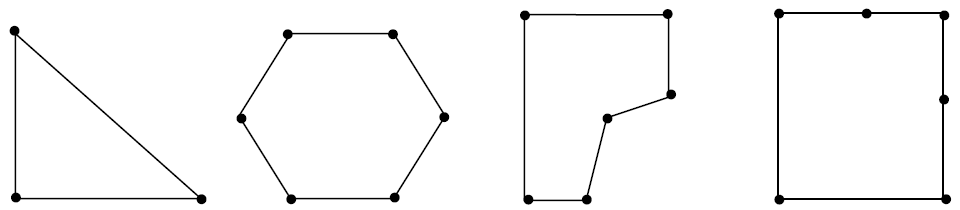
\includegraphics[width=0.70\textwidth]{images/arbitrary_polygons.png}
\end{block}
\vspace{0.5cm}
\begin{block}{3D convex polyhedra}
\centering
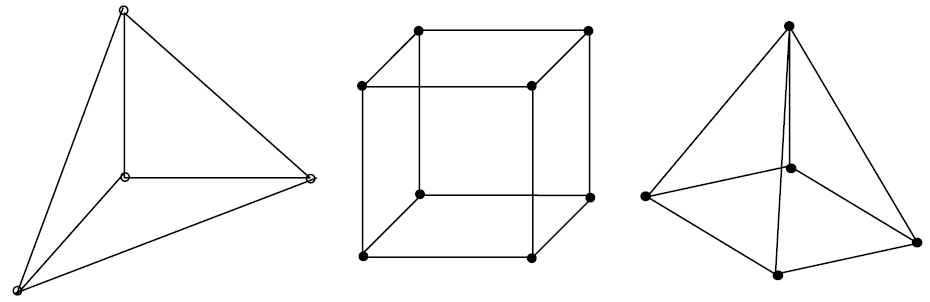
\includegraphics[width=0.70\textwidth]{images/arbitrary_polyhedra.png}
\end{block}
\end{frame}
% --------------------------------------------
\begin{frame}[t]\frametitle{Finite element architecture}
\begin{block}{Mass Matrix - element $K$}
\begin{equation*}
{\bf M}^K = \int_{K} d\vec{r} \, \lambda (\vec{x}) \, \lambda^T (\vec{x})  =  \sum\displaylimits_{q=1}^{N_q^K} w_q^K \, \lambda (\vec{x}_q^K) \, \lambda^T (\vec{x}_q^K) 
\end{equation*}
\end{block}
\begin{block}{Advection Matrix - element $K$}
\begin{equation*}
{\bf G}^K = \int_{K} d\vec{r} \, \vec{\nabla} \lambda (\vec{x}) \, \lambda^T (\vec{x}) = \sum\displaylimits_{q=1}^{N_q^K}  w_q^K \, \vec{\nabla} \lambda (\vec{x}_q^K) \, \lambda^T (\vec{x}_q^K) 
\end{equation*}
\end{block}
\begin{block}{Surface Matrix - face $f$ for element $K$}
\begin{equation*}
{\bf N}_f^K = \int_{f} ds \, \lambda (\vec{x}) \, \lambda^T (\vec{x})  = \sum\displaylimits_{q=1}^{N_f}  w_q^f \, \lambda (\vec{x}_q^f) \, \lambda^T (\vec{x}_q^f) 
\end{equation*}
\end{block}
\end{frame}
% --------------------------------------------
%%%%%%%%%%%%%%%%%%%
\subsection{Linear Basis Functions on Polygons}
%%%%%%%%%%%%%%%%%%%
% --------------------------------------------
\begin{frame}[t]\frametitle{Linear Basis Functions - Generalized Barycentric Coordinates}
\centering
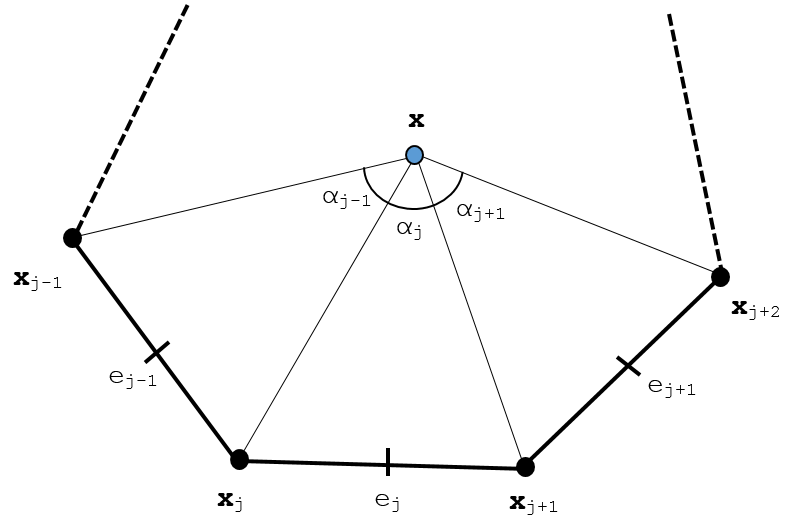
\includegraphics[width=0.35\textwidth]{images/ref_polygon.png}
\only<1>{
\begin{block}{Basis Function Properties - Barycentric Coordinates}{\small
$\lambda_i$ - linear basis function located at vertex $i$ \vspace{0.25cm}
\vspace{-1mm}
	\begin{enumerate}
	\item Positivity*: $\lambda_i \geq 0$ \vspace{1mm}
	\item Partition of Unity: $\sum_i \lambda_i = 1$ \vspace{1mm}
	\item Affine combination: $\sum_i \vec{x}_i \lambda_i (\vec{x}) = \vec{x}$ \vspace{1mm}
	\item Lagrange property: $\lambda_i (\vec{x}_j) = \delta_{ij}$ 
	\item Piecewise boundary linearity: $\lambda_j ((1-\mu ) \vec{x}_j  + \mu \vec{x}_{j+1})  = (1-\mu ) \lambda_j (\vec{x}_j ) + \mu \lambda_j (\vec{x}_{j+1} )$
	\end{enumerate}
\vspace{1mm}
*convex polygons
}\end{block}
}
\only<2>{
\begin{block}{Linear basis functions that we consider}
	\begin{enumerate}
	\item Wachspress rational coordinates*
	\item Piecewise linear (PWL) coordinates*
	\item Mean value coordinates
	\item Maximum entropy coordinates
	\end{enumerate}
\vspace{2mm}
*have been previously analyzed for transport problems
\end{block}
}
\end{frame}
% --------------------------------------------
\begin{frame}[t]\frametitle{Wachspress Rational Functions}

\end{frame}
% --------------------------------------------
\begin{frame}[t]\frametitle{Piecewise Linear Functions}

\end{frame}
% --------------------------------------------
\begin{frame}[t]\frametitle{Mean Value Coordinates}

\end{frame}
% --------------------------------------------
\begin{frame}[t]\frametitle{Maximum Entropy Coordinates}

\end{frame}
% --------------------------------------------
\begin{frame}[t]\frametitle{Summary of the Linear Basis Functions}

\end{frame}
% --------------------------------------------
%%%%%%%%%%%%%%%%%%%
\subsection{Quadratic Basis Functions on Polygons}
%%%%%%%%%%%%%%%%%%%
% --------------------------------------------
\begin{frame}[t]\frametitle{Quadratic Serendipity Basis Functions on 2D Polygons}
\begin{block}{}
\begin{enumerate}
	\item <1-> Form the linear barycentric functions - \{$\lambda_i$\}
	\item <2-> Construct the pairwise products -  \{$\mu_{ab}$\}
	\item <3-> Eliminate the interior nodes to form a serendipity basis - \{$\xi_{ij}$\}
\end{enumerate}
\end{block}
\vspace{1cm}
\begin{columns}[c]
\column{0.28\textwidth}
\centering
\only<1-3>{
{}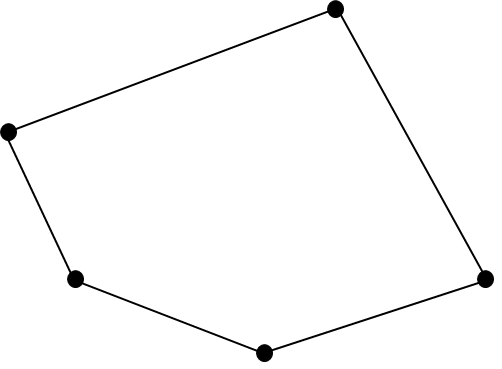
\includegraphics[width=0.9\columnwidth]{images/rand_linear.png} \\
\{$\lambda_i$\} \\
Linear
}
\column{0.08\textwidth}
\only<2-3>{
$\longrightarrow$
}
\column{0.28\textwidth}
\centering
\only<2-3>{
{}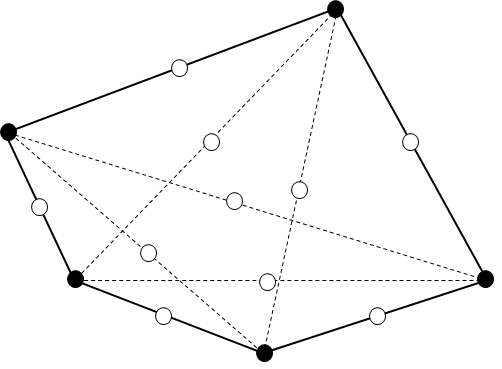
\includegraphics[width=0.9\columnwidth]{images/rand_quadratic.png} \\
\{$\mu_{ab}$\} \\
Quadratic
}
\column{0.08\textwidth}
\only<3>{
$\longrightarrow$
}
\column{0.28\textwidth}
\centering
\only<3>{
{}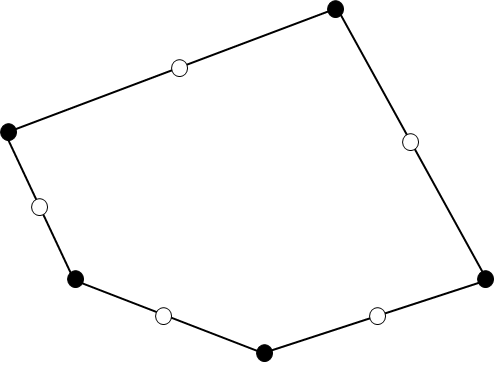
\includegraphics[width=0.9\columnwidth]{images/rand_serendipity.png} \\
\{$\xi_{ij}$\} \\
Serendipity
}
\end{columns}
\end{frame}
% --------------------------------------------
\begin{frame}[t]\frametitle{Pairwise products of the barycentric basis functions - $\mu_{ab} = \lambda_a \lambda_b$}
\only<1>{
\centering
{}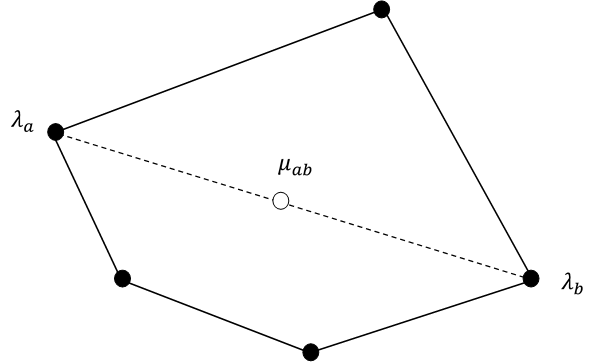
\includegraphics[width=0.75\columnwidth]{images/rand_quad_ab.png} 
}
\only<2>{
\begin{block}{Necessary Constraints}
\begin{columns}
\column{0.62\textwidth}
\begin{equation*}
\sum_{aa \in V} \mu_{aa} + \sum_{ab \in E \cup D} 2 \mu_{ab} = 1
\end{equation*}
\begin{equation*}
\sum_{aa \in V} \vec{x}_{aa} \mu_{aa} + \sum_{ab \in E \cup D} 2 \vec{x}_{ab} \mu_{ab} = \vec{x}
\end{equation*}
\begin{equation*}
\sum_{aa \in V} \vec{x}_{a} \vec{x}_{a}^T \mu_{aa} + \sum_{ab \in E \cup D} \left(  \vec{x}_{a} \vec{x}_{b}^T + \vec{x}_{b} \vec{x}_{a}^T  \right) \mu_{ab} = \vec{x} \vec{x}^{T}
\end{equation*}
\column{0.03\textwidth}
\column{0.35\textwidth}
{\small
$V$ - vertex nodes \\
$E$ - face midpoint nodes \\
$D$ - interior diagonal nodes \\ \vspace{3mm}
$V+E+D = n + n + \frac{n(n-3)}{2}$
}
\end{columns}
\end{block}
\begin{block}{Further Notation/Notes}
\begin{equation*}
\vec{x}_{ab} = \frac{\vec{x}_{a} + \vec{x}_{b}}{2}, \qquad \mu_{ab} = \lambda_a \lambda_b
\end{equation*}
\vspace{0.4cm}
\begin{equation*}
\mu^{K}_{ab}(\vec{r}) = 0, \qquad \left\{ ab \in D , \, \vec{r} \in \partial K  \right\}
\end{equation*}
\end{block}
}
\end{frame}
% --------------------------------------------
\begin{frame}[t]\frametitle{Eliminate interior nodes to form Serendipity basis}

\end{frame}
% --------------------------------------------
\begin{frame}[t]\frametitle{Example Images}

\end{frame}
% --------------------------------------------
%%%%%%%%%%%%%%%%%%%
\subsection{Linear Basis Functions on Polyhedra}
%%%%%%%%%%%%%%%%%%%
% --------------------------------------------
\setbeamerfont{frametitle}{size=\large}
\begin{frame}[t]{Linear Basis Functions on 3D Polyhedra}
\begin{block}{Linear basis functions and convex polyhedra only for 3D}{\small
\begin{itemize}
\item The 2D quadratic serendipity formulation is more arduous in 3D
\item Intercell coupling is not straightforward for concave polyhedra
\item Focus on 3D PWL functions
\item Focus on 3D parallelepipeds and extruded convex polygons (convex prisms)
\end{itemize}}
\end{block}
\begin{block}{3D PWL basis functions}{\small
\begin{equation*}
b_i (\vec{x})  = t_i  (\vec{x})  + \sum_{f=1}^{F_i} \beta_f^i  t_f (\vec{x}) + \alpha_i t_c  (\vec{x}) 
\end{equation*}
}\end{block}
\begin{block}{}{\footnotesize
$t_i$ - standard 3D linear function for a tet $(i,i+1,f_c,K_c)$; 1 at vertex $i$, linearly decreases to 0 to the cell center, each adjoining face center, and each adjoining vertex\\ \vspace{0.5mm}
$t_c$ - 3D tent function; 1 at cell center, linearly decreases to 0 at all vertices and face centers \\ \vspace{0.5mm}
$t_f$ - face tent function; 1 at face center, linearly decreases to 0 at each face vertex and cell center\\ \vspace{0.5mm}
$\alpha_i = \frac{1}{N_V}$ - weight parameter for vertex $i$\\ \vspace{0.5mm}
$\beta_f^i = \frac{1}{N_f}$ - weight parameter for face $f$ touching vertex $i$
}\end{block}
\end{frame}
% --------------------------------------------
%%%%%%%%%%%%%%%%%%%
\subsection{Results}
%%%%%%%%%%%%%%%%%%%
% --------------------------------------------
\begin{frame}[t]\frametitle{Results Summary}
\begin{block}{}
\begin{enumerate}
\item Linear and quadratic basis functions capture the thick diffusion limit.
\item Linear basis functions capture exactly-linear transport solutions.
\item Quadratic basis functions capture exactly-quadratic transport solutions.
\item Convergence rate analysis using the Method of Manufactured Solutions. 
\item Convergence rate analysis bound by the solution regularity.
\end{enumerate}
\end{block}
\end{frame}
% --------------------------------------------
\begin{frame}[t]\frametitle{Thick Diffusion Limit}

\end{frame}
% --------------------------------------------
\begin{frame}[t]\frametitle{Exactly-Linear Transport Solutions}

\end{frame}
% --------------------------------------------
\begin{frame}[t]\frametitle{Exactly-Quadratic Transport Solutions}

\end{frame}
% --------------------------------------------
\begin{frame}[t]
\only<1>
{
\frametitle{Convergence Rate Analysis by MMS}
{\small
\begin{block}{Sinusoid Solution}
\begin{equation*}
\begin{aligned}
\Psi_s (x,y) = &\sin(\nu  \frac{\pi x}{L_x}) \sin(\nu  \frac{\pi y}{L_y}) \\ 
\Phi_s (x,y) = 2 \pi &\sin(\nu  \frac{\pi x}{L_x}) \sin(\nu  \frac{\pi y}{L_y})
\end{aligned} 
\end{equation*}
\begin{itemize}
\item Cartesian, triangular and Voronoi polygon meshes
\item Wachspress, PWL, MV, and MAXENT
\end{itemize}
\end{block}
\begin{block}{Localized Gaussian Solution}
\begin{equation*}
\begin{aligned}
\Psi_g (x,y) = & \frac{x (L_x - x)}{L_x^2} \frac{y (L_y - y)}{L_y^2} \exp(-\frac{(x-x_0)^2 + (y-y_0)^2}{L_x L_y}) \\ 
\Phi_g (x,y) = 2 \pi &\frac{x (L_x - x)}{L_x^2} \frac{y (L_y - y)}{L_y^2} \exp(-\frac{(x-x_0)^2 + (y-y_0)^2}{L_x L_y})
\end{aligned} 
\end{equation*}
\begin{itemize}
\item Use spatial Adaptive Mesh Refinement (AMR)
\item PWL, MV, and MAXENT
\end{itemize}
\end{block}
}
}
\only<2>
{
\frametitle{Cartesian Sinusoid MMS Results}
\vspace{1.5cm}
\begin{columns}
\column{0.40\textwidth}
{}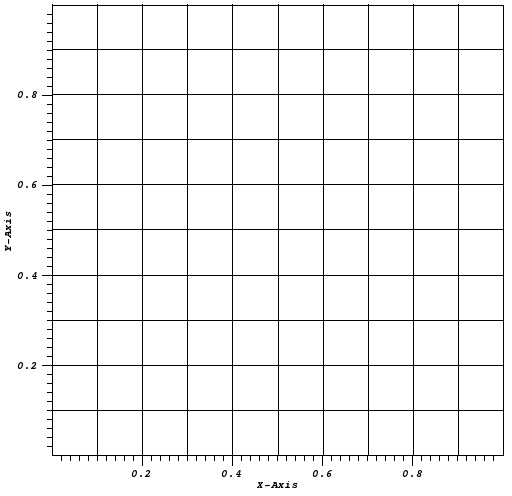
\includegraphics[width=0.8\columnwidth]{images/cart_mesh.jpg}
\column{0.60\textwidth}
{}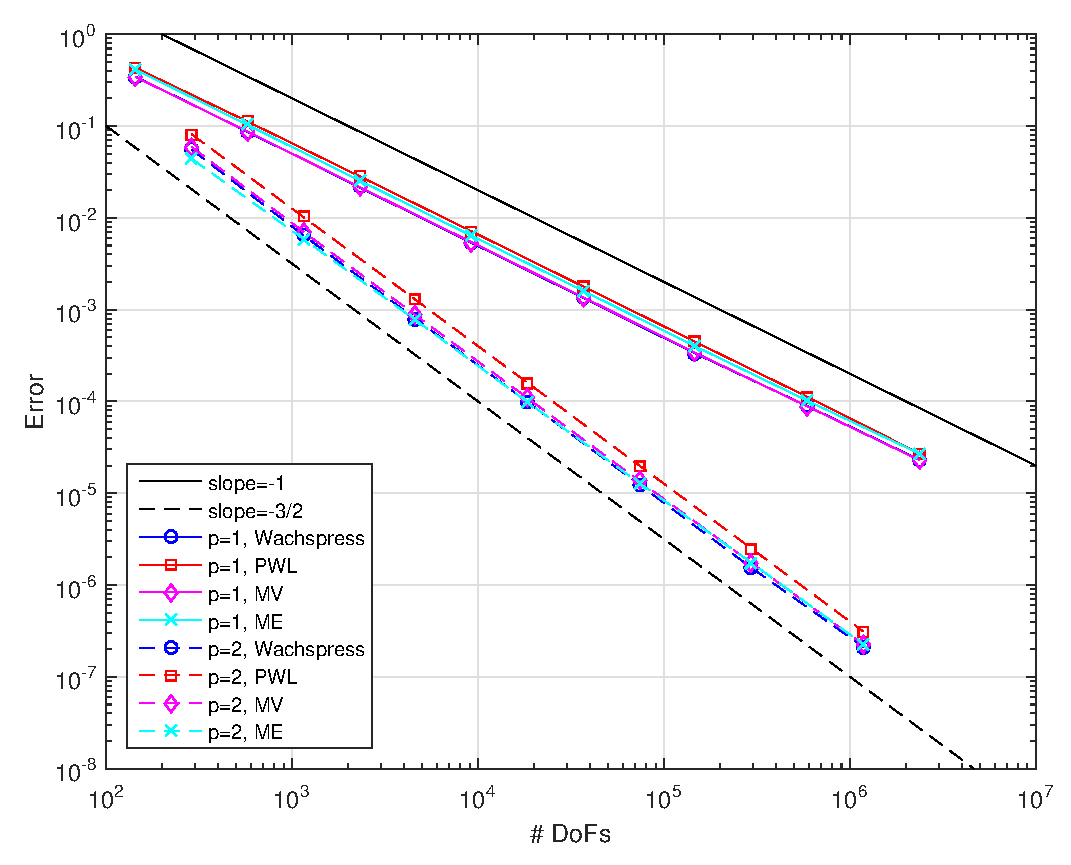
\includegraphics[width=0.9\columnwidth]{images/TransMMS_Sine_cart_err.eps}
\end{columns}
}
\only<3>
{
\frametitle{Triangular Sinusoid MMS Results}
\vspace{1.5cm}
\begin{columns}
\column{0.40\textwidth}
{}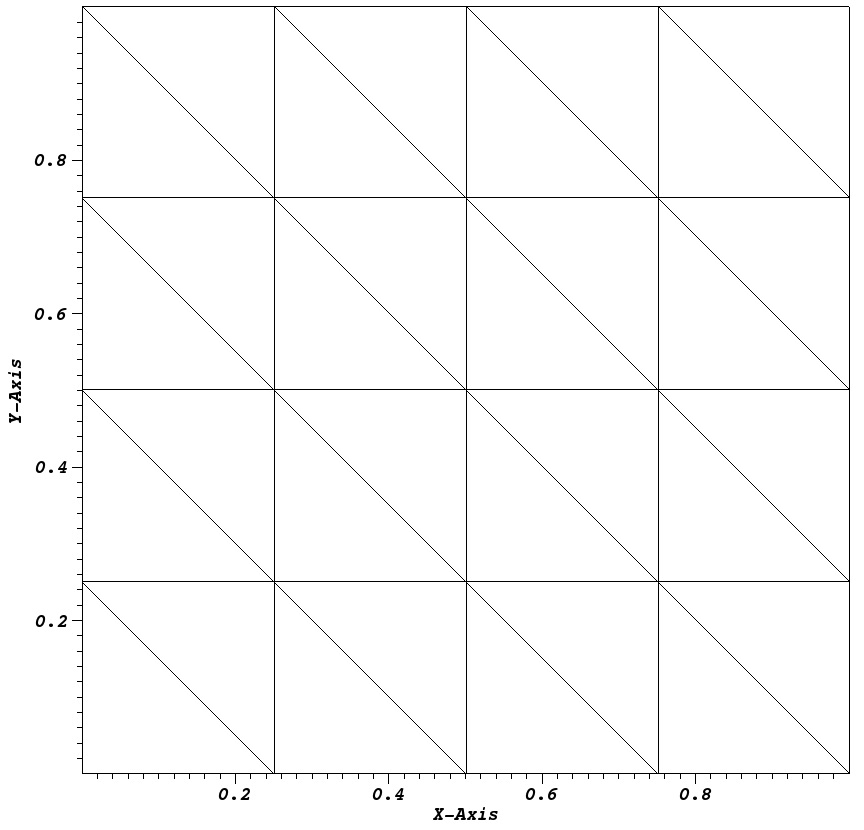
\includegraphics[width=0.8\columnwidth]{images/tri_mesh.jpg}
\column{0.60\textwidth}
{}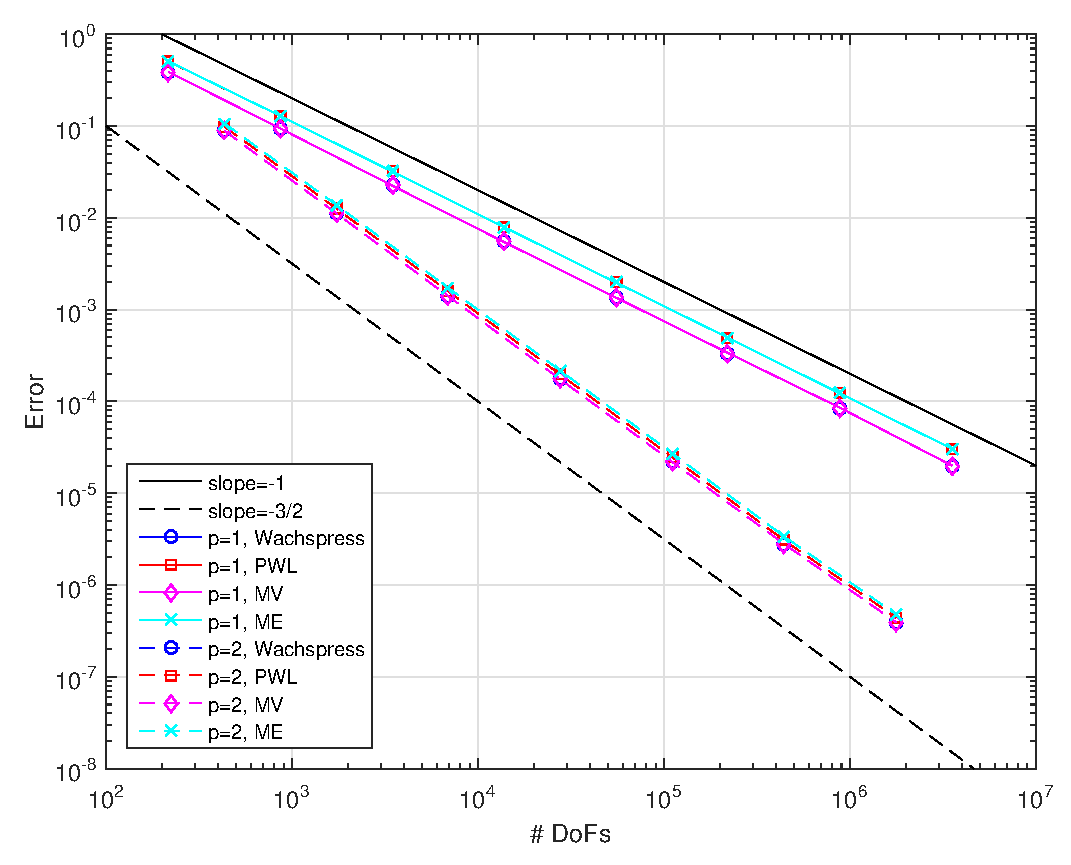
\includegraphics[width=0.9\columnwidth]{images/TransMMS_Sine_tri_err.eps}
\end{columns}
}
\only<4>
{
\frametitle{Polygonal Sinusoid MMS Results}
\vspace{1.5cm}
\begin{columns}
\column{0.40\textwidth}
{}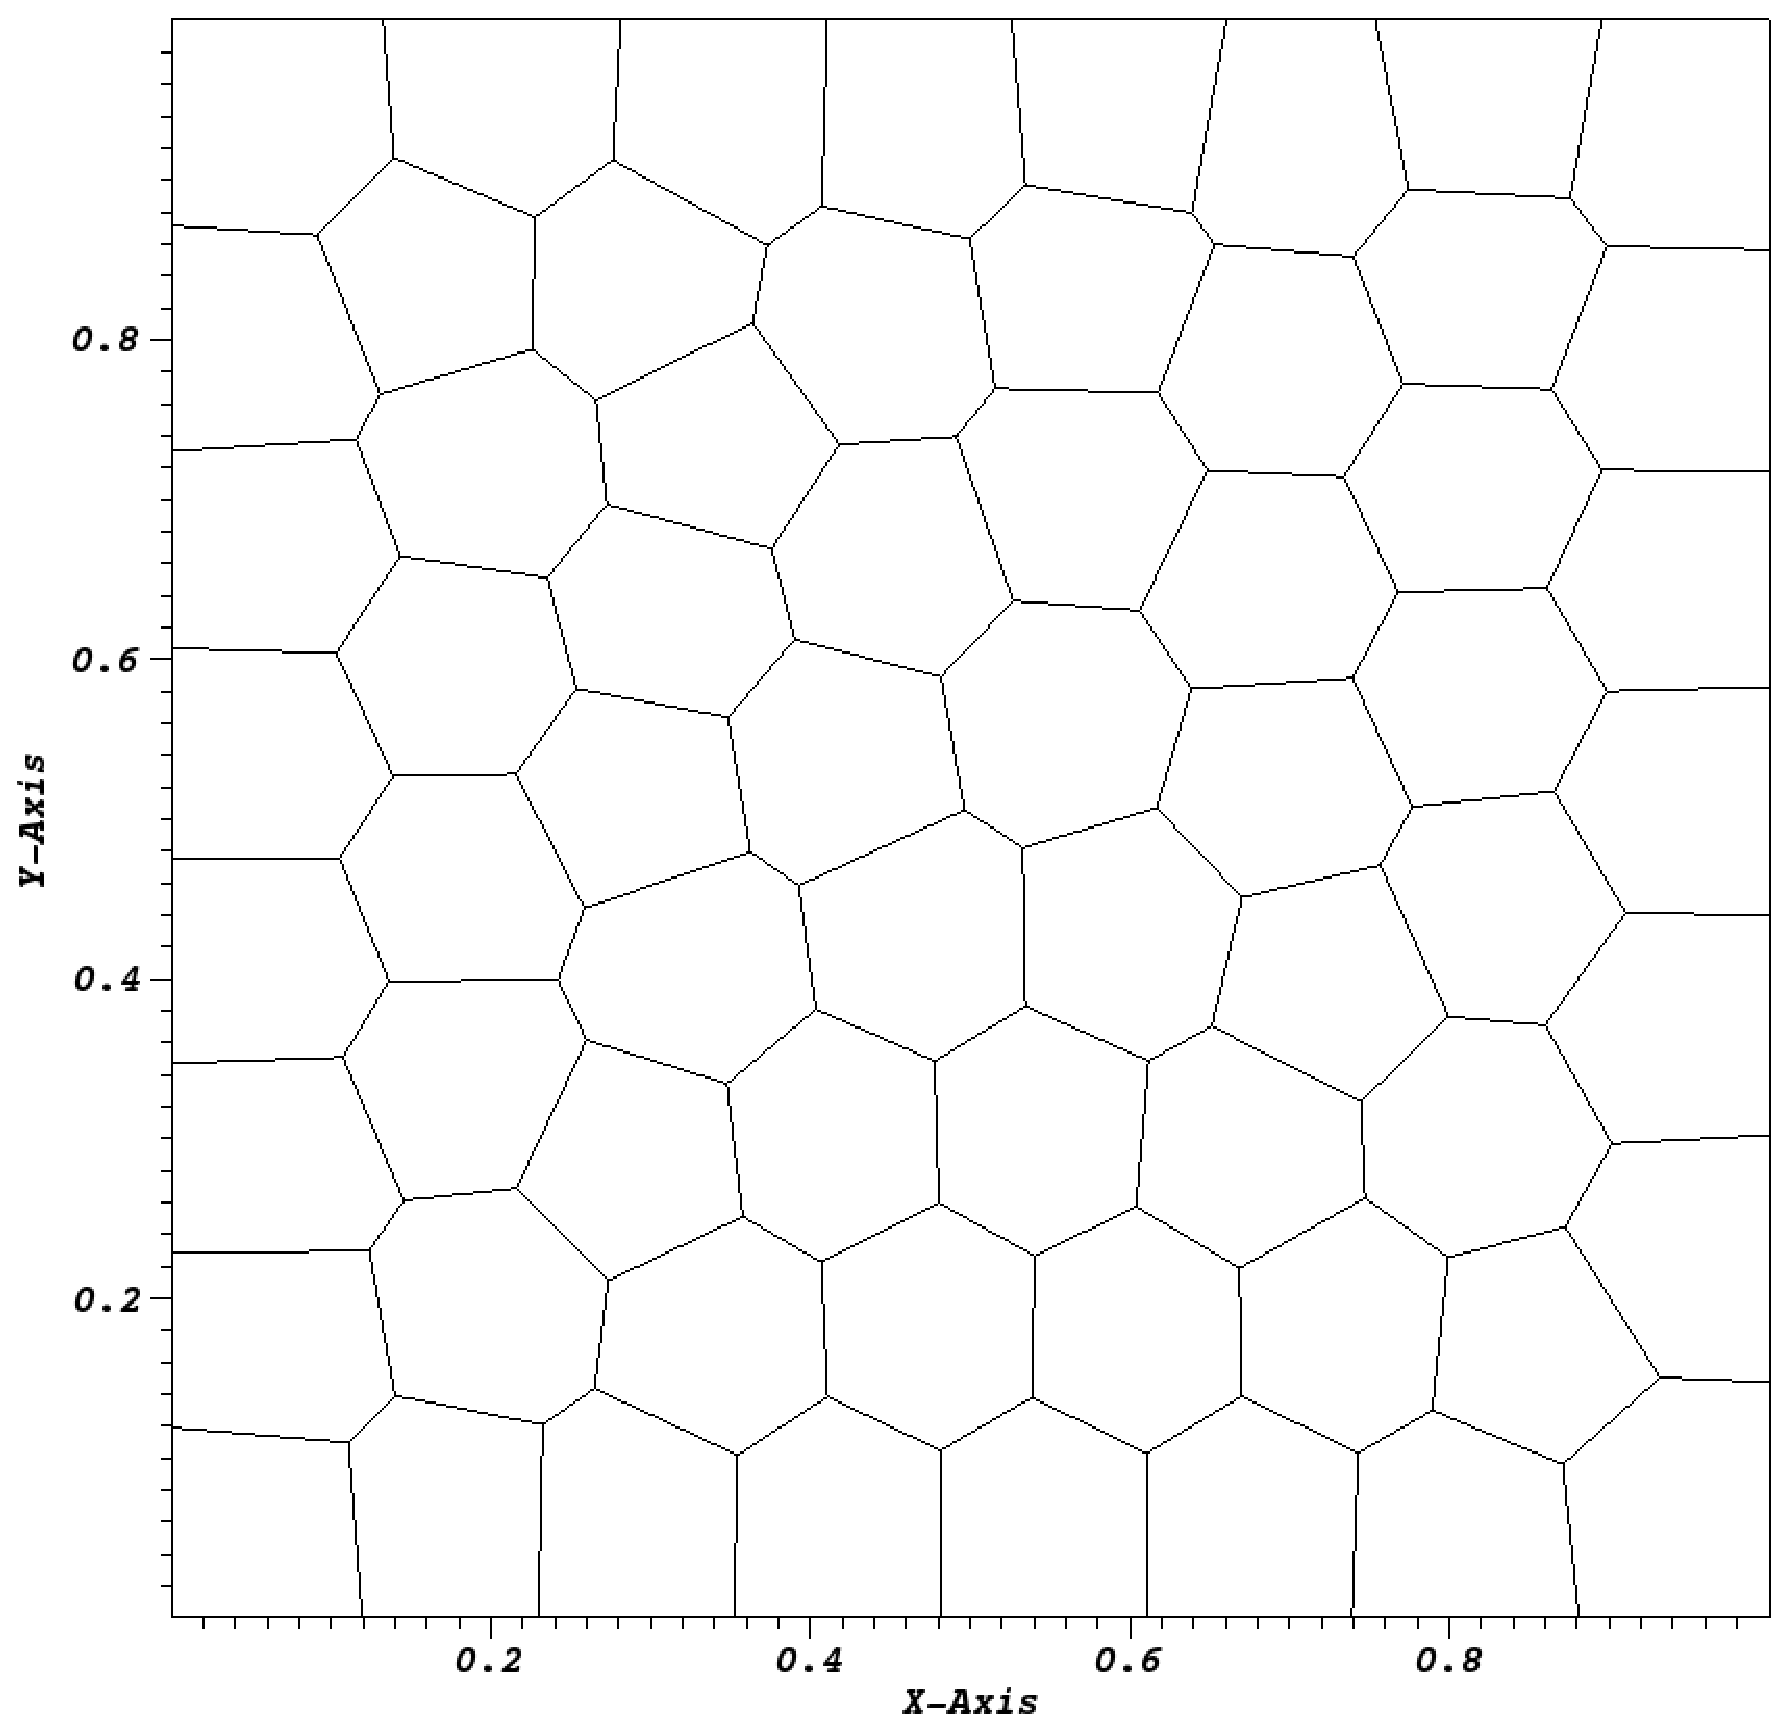
\includegraphics[width=0.8\columnwidth]{images/PolyMesh_mesh.eps}
\column{0.60\textwidth}
{}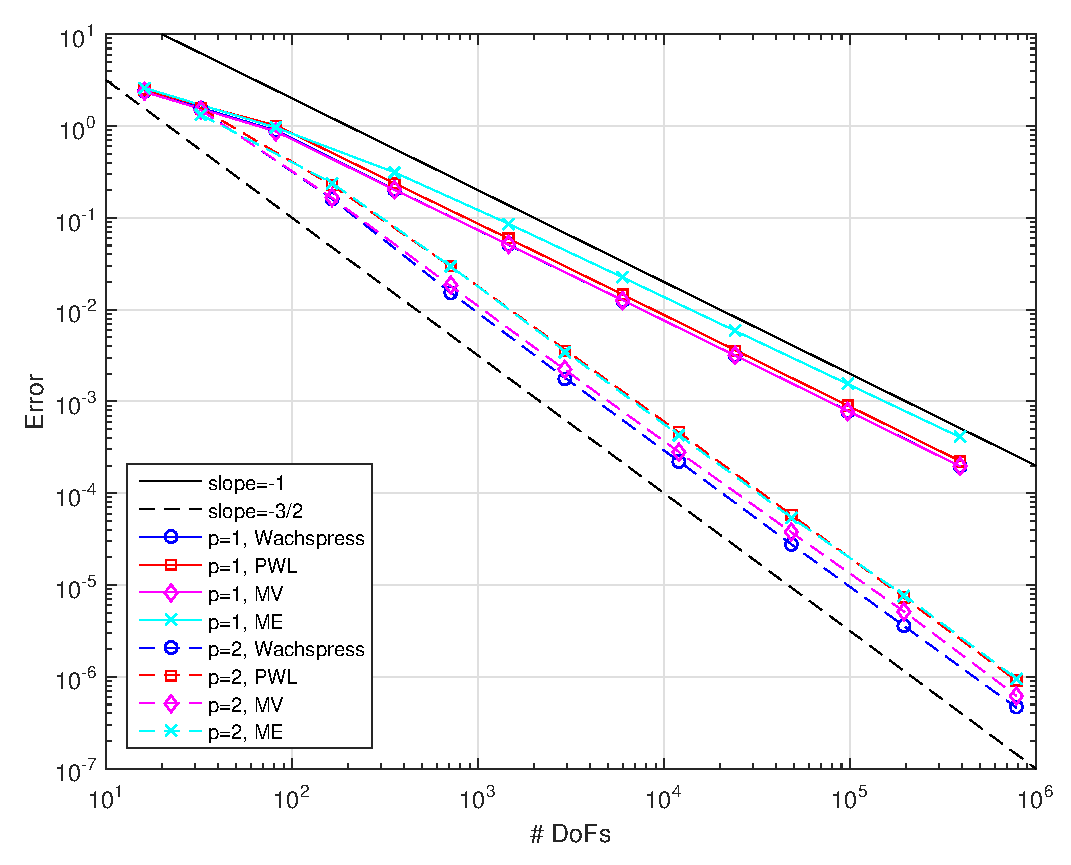
\includegraphics[width=0.9\columnwidth]{images/TransMMS_Sine_poly_err.eps}
\end{columns}
}
\only<5>
{
\frametitle{\footnotesize Gaussian AMR - Linear ME cycle 15 (left) and quadratic ME cycle 08 (right)}
\begin{columns}
\column{0.50\textwidth}
\centering
{}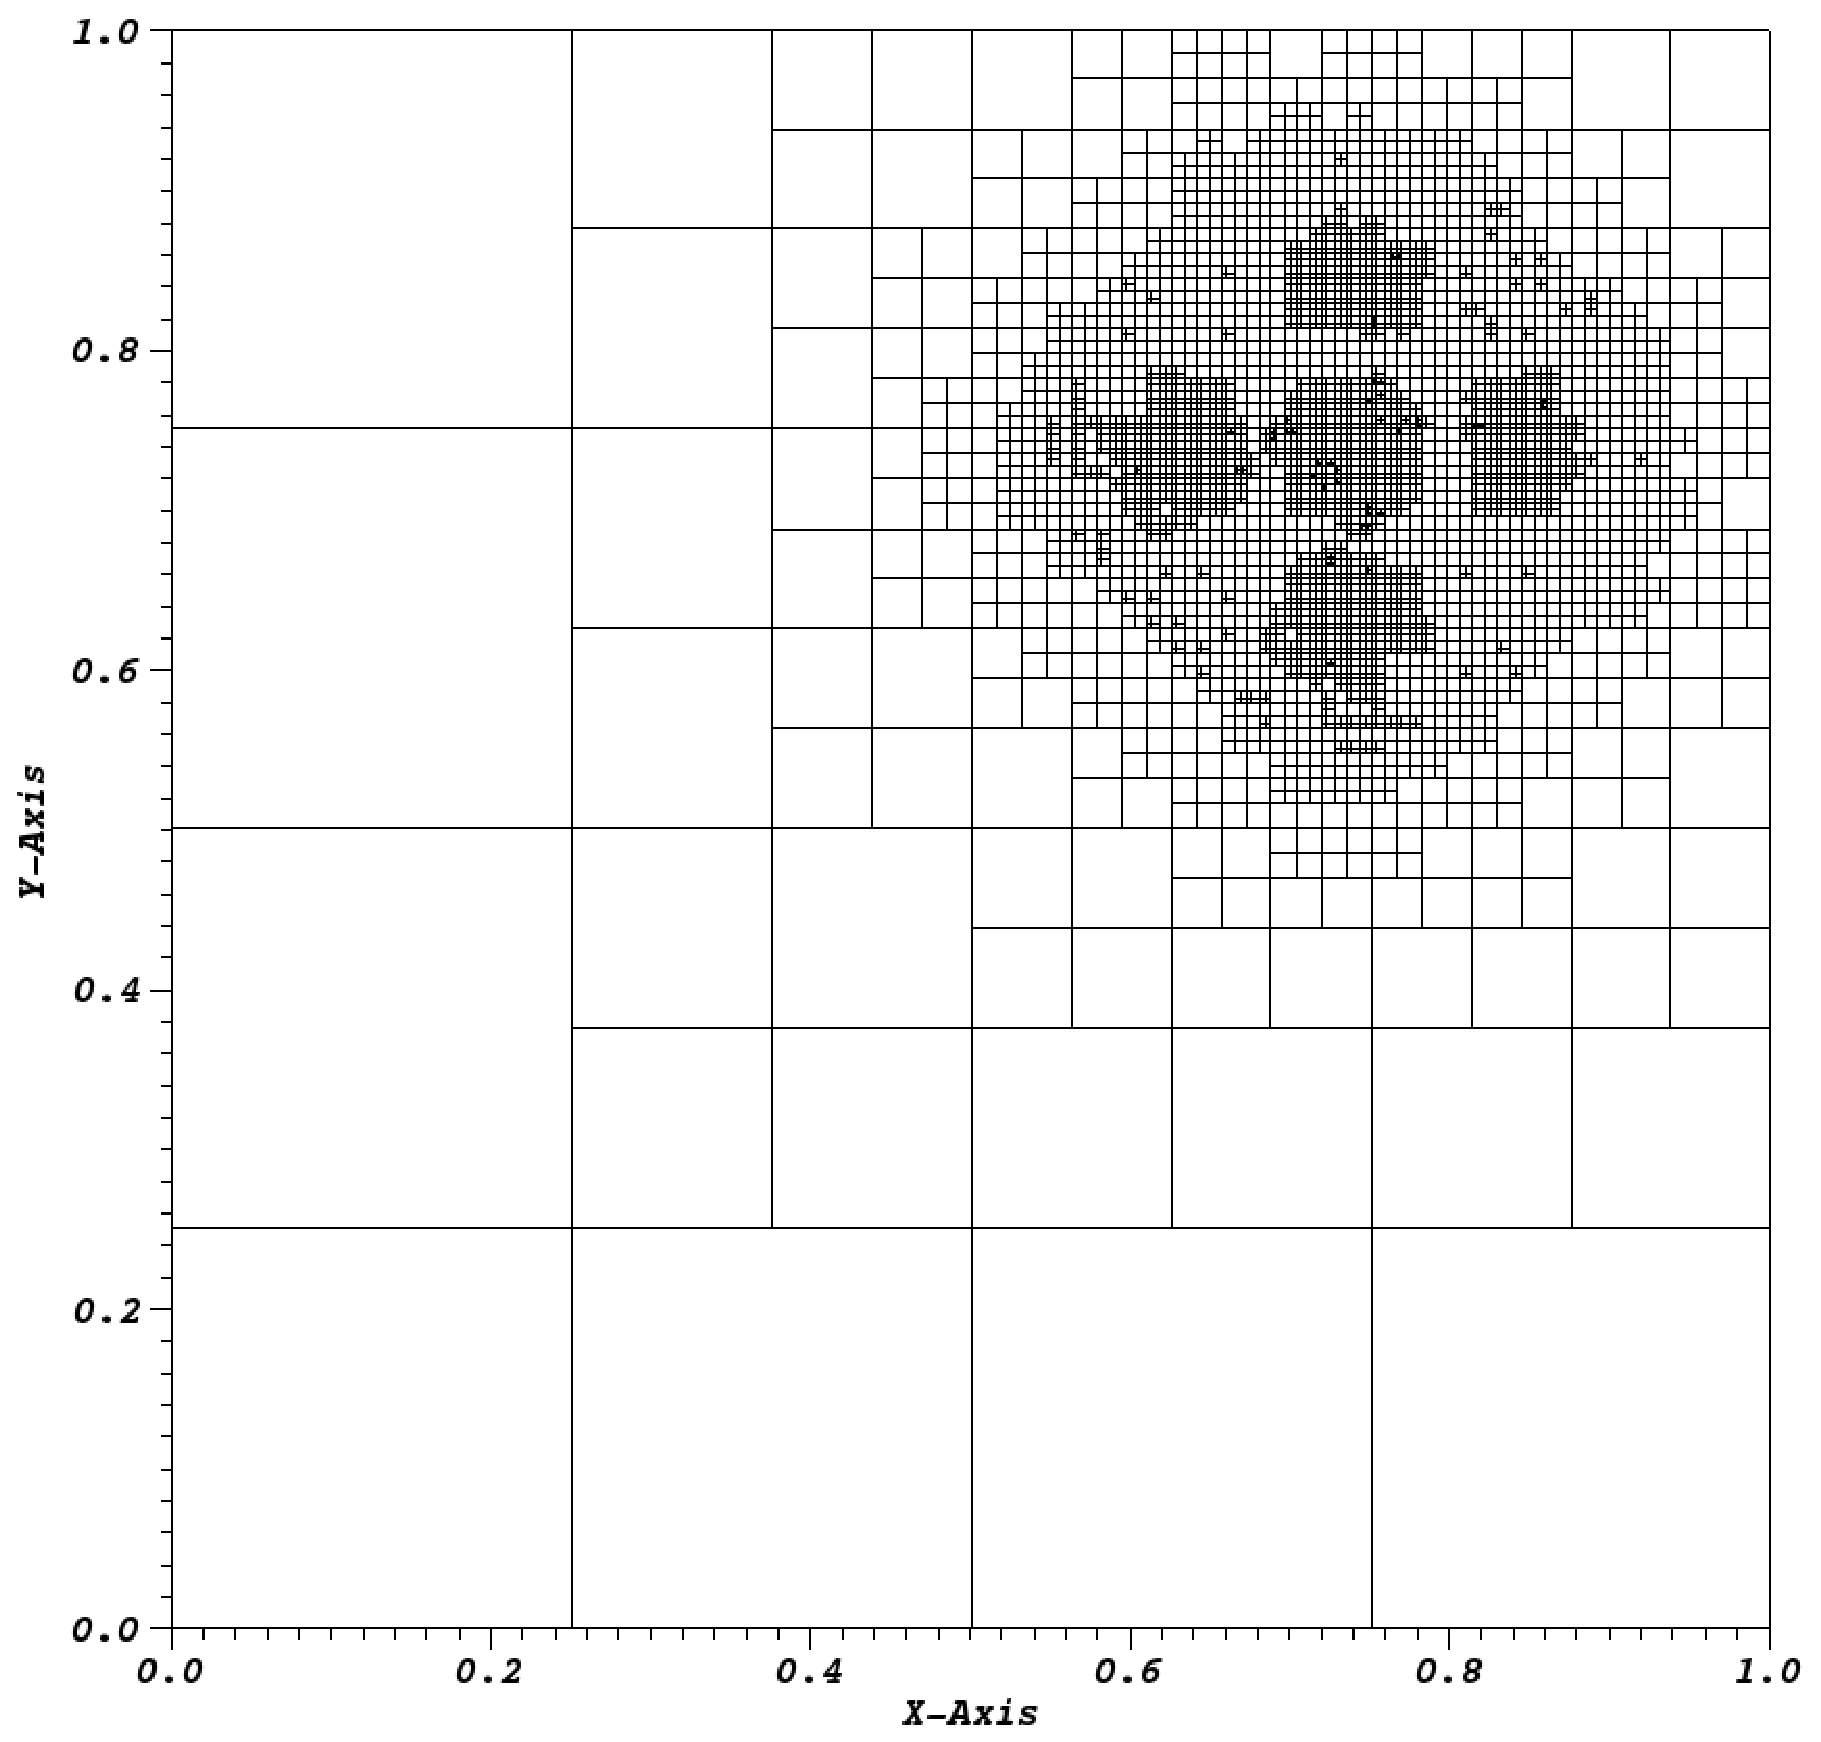
\includegraphics[width=0.70\columnwidth]{images/ME1_cart_Irr=1_tol=0.2_cyc15_mesh.eps} \\
{}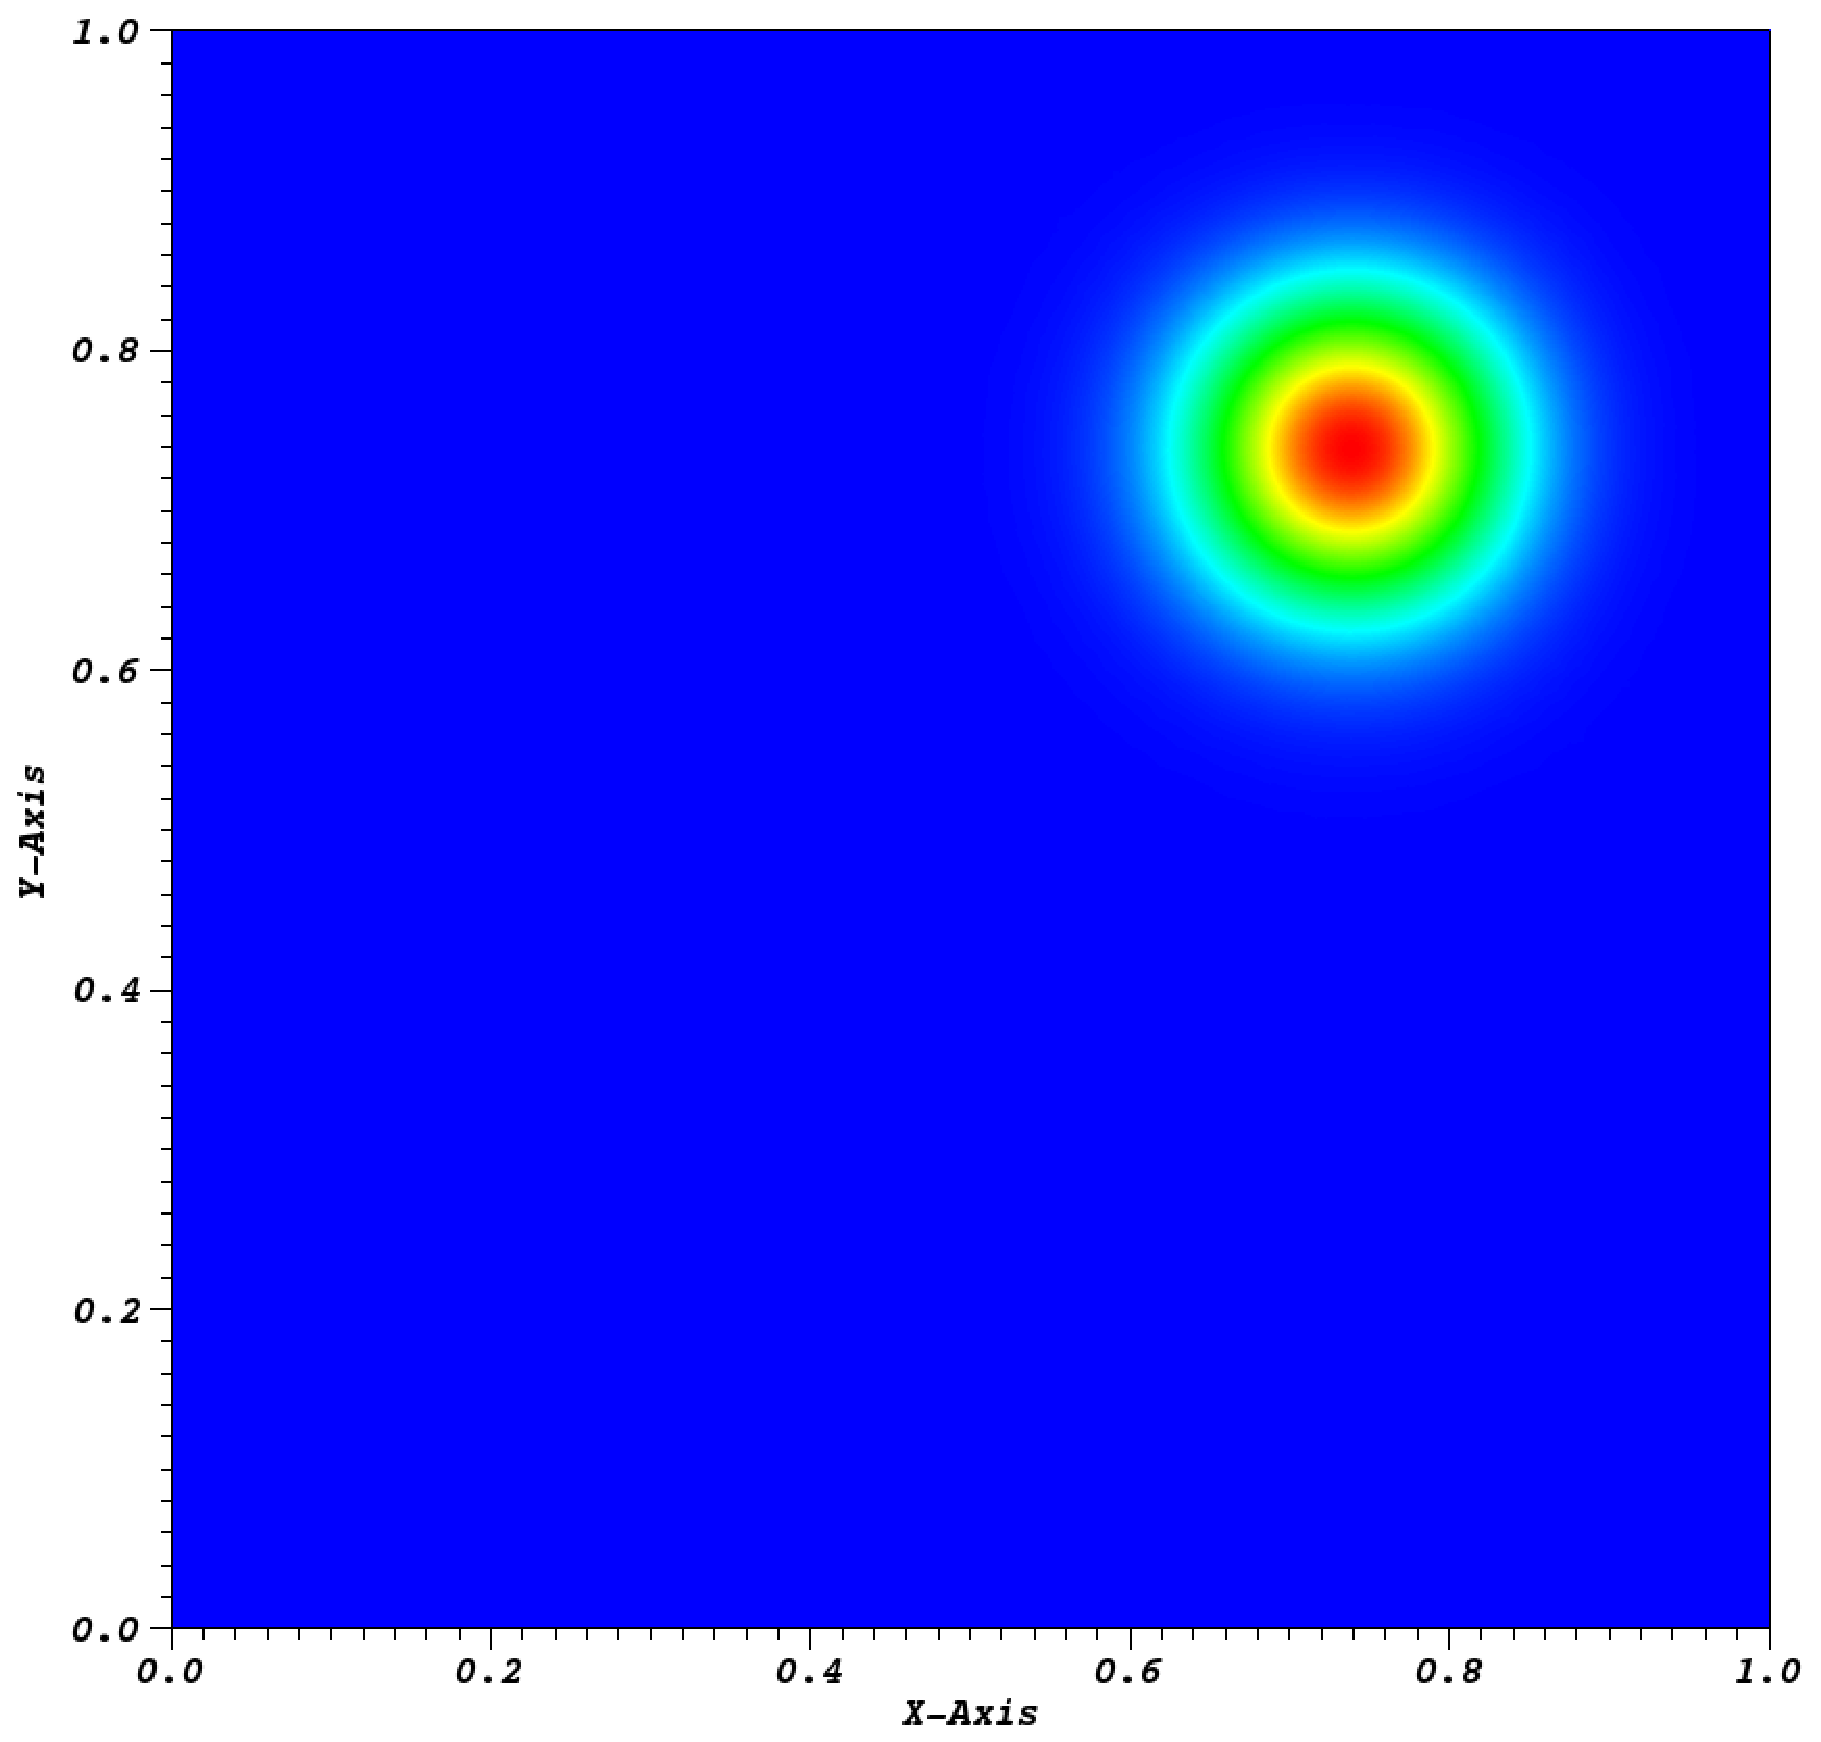
\includegraphics[width=0.70\columnwidth]{images/ME1_cart_Irr=1_tol=0.2_cyc15_sol.eps}
\column{0.50\textwidth}
\centering
{}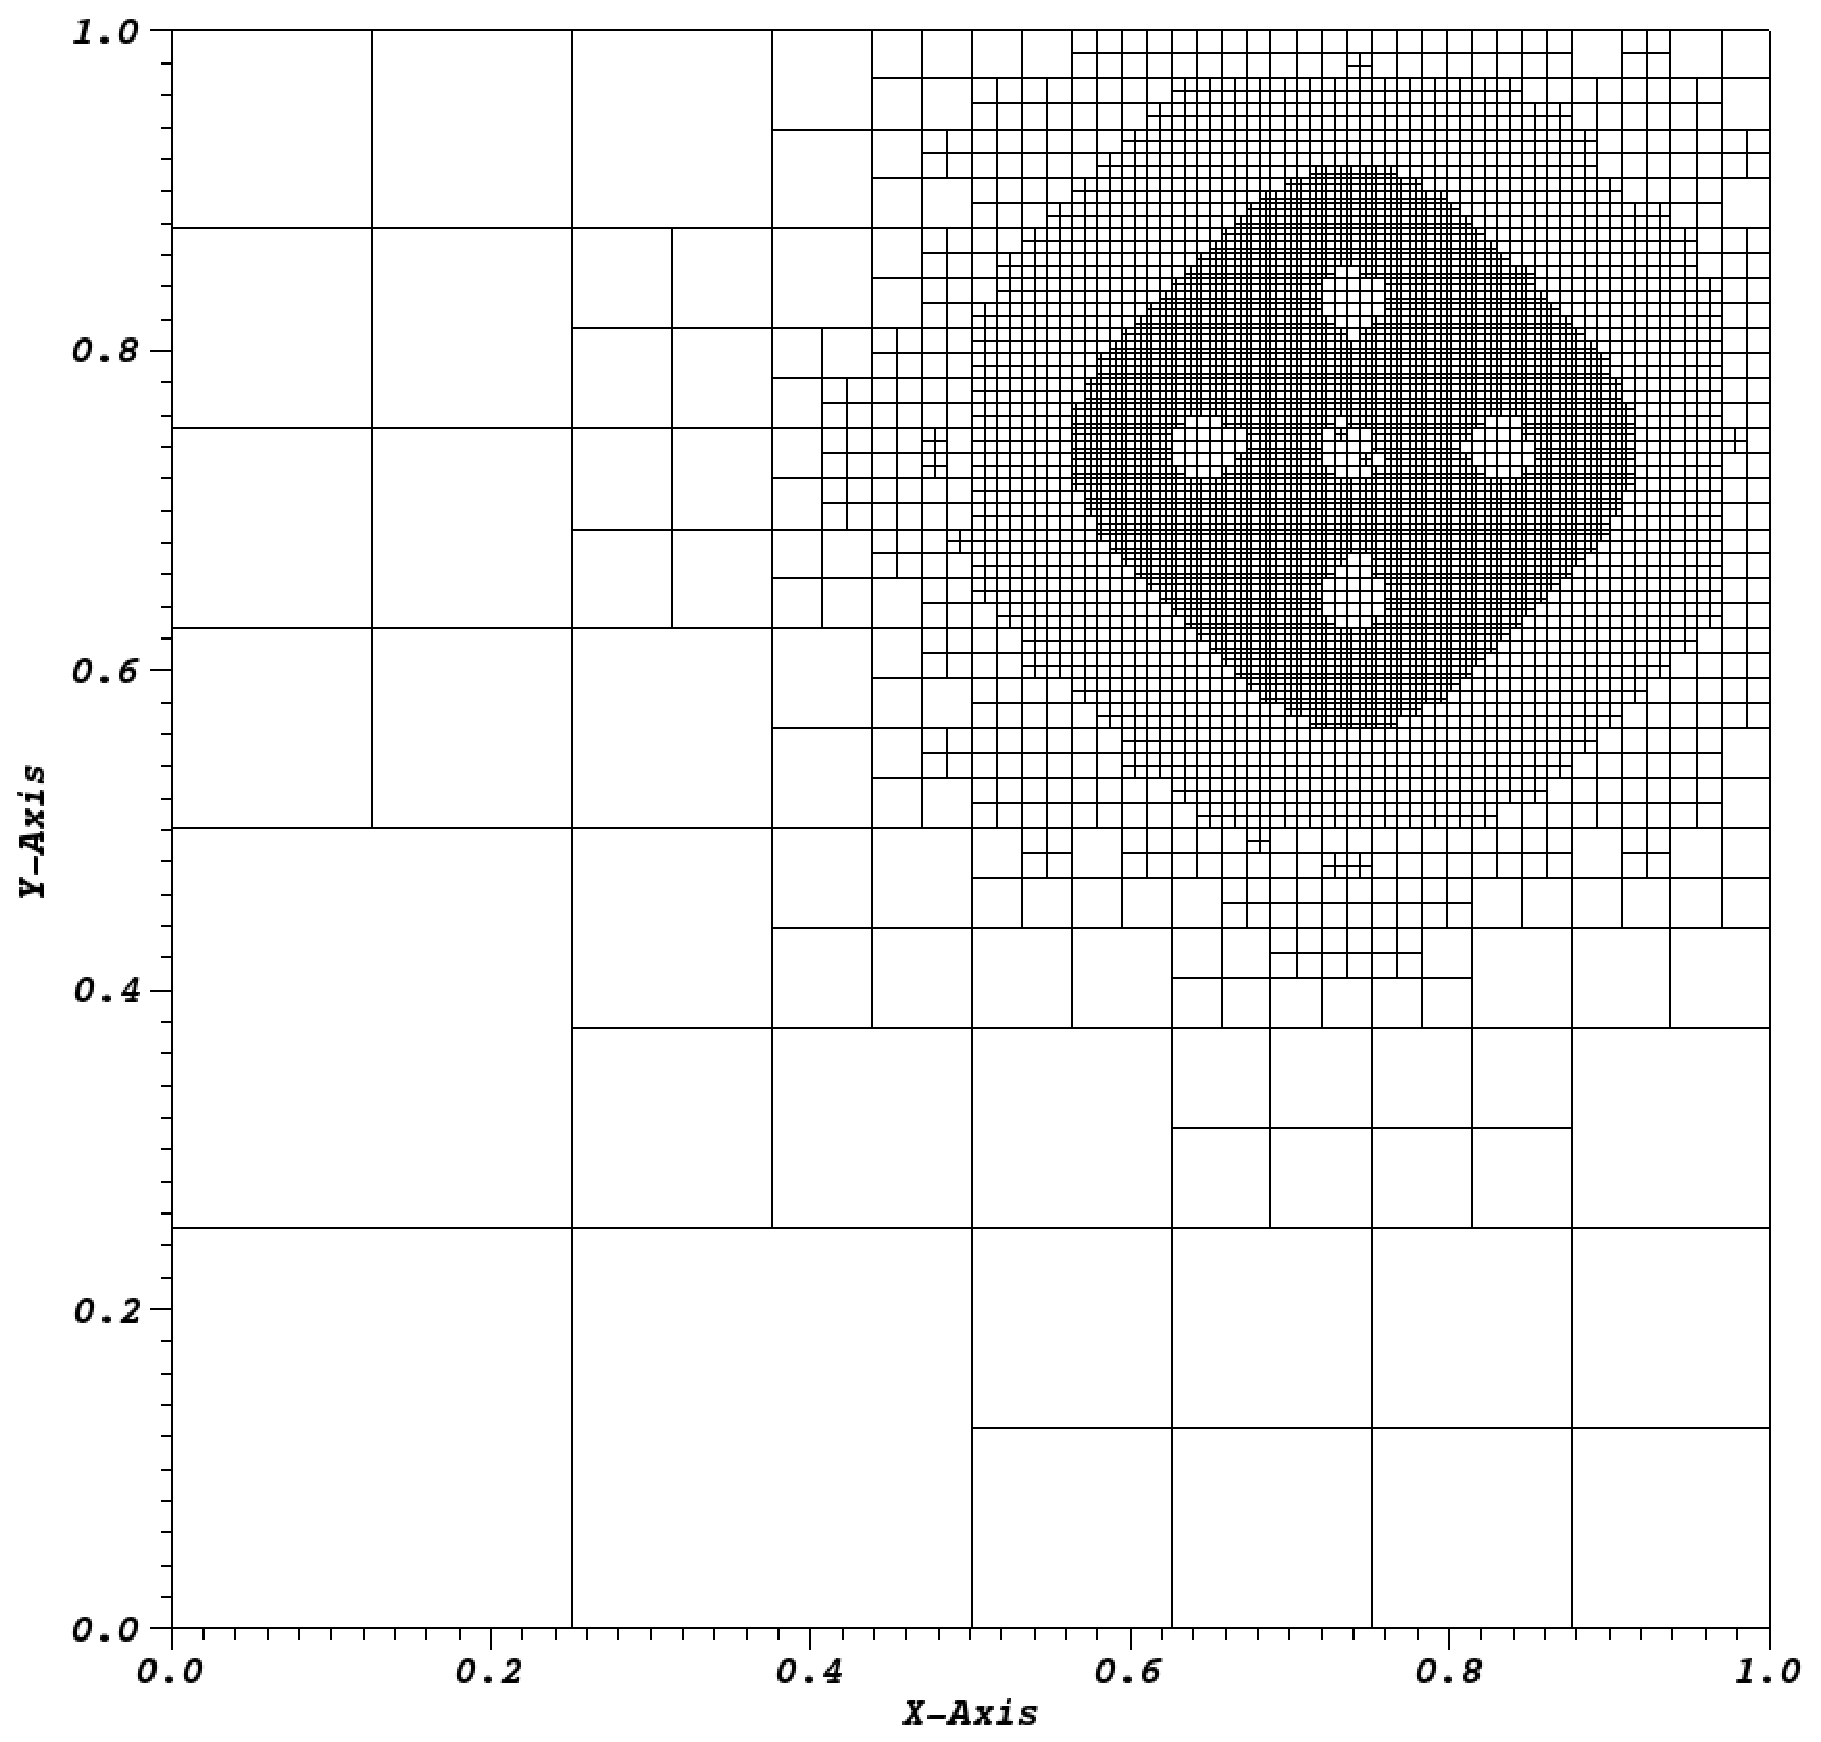
\includegraphics[width=0.70\columnwidth]{images/ME2_cart_Irr=1_tol=0.1_cyc08_mesh.eps} \\
{}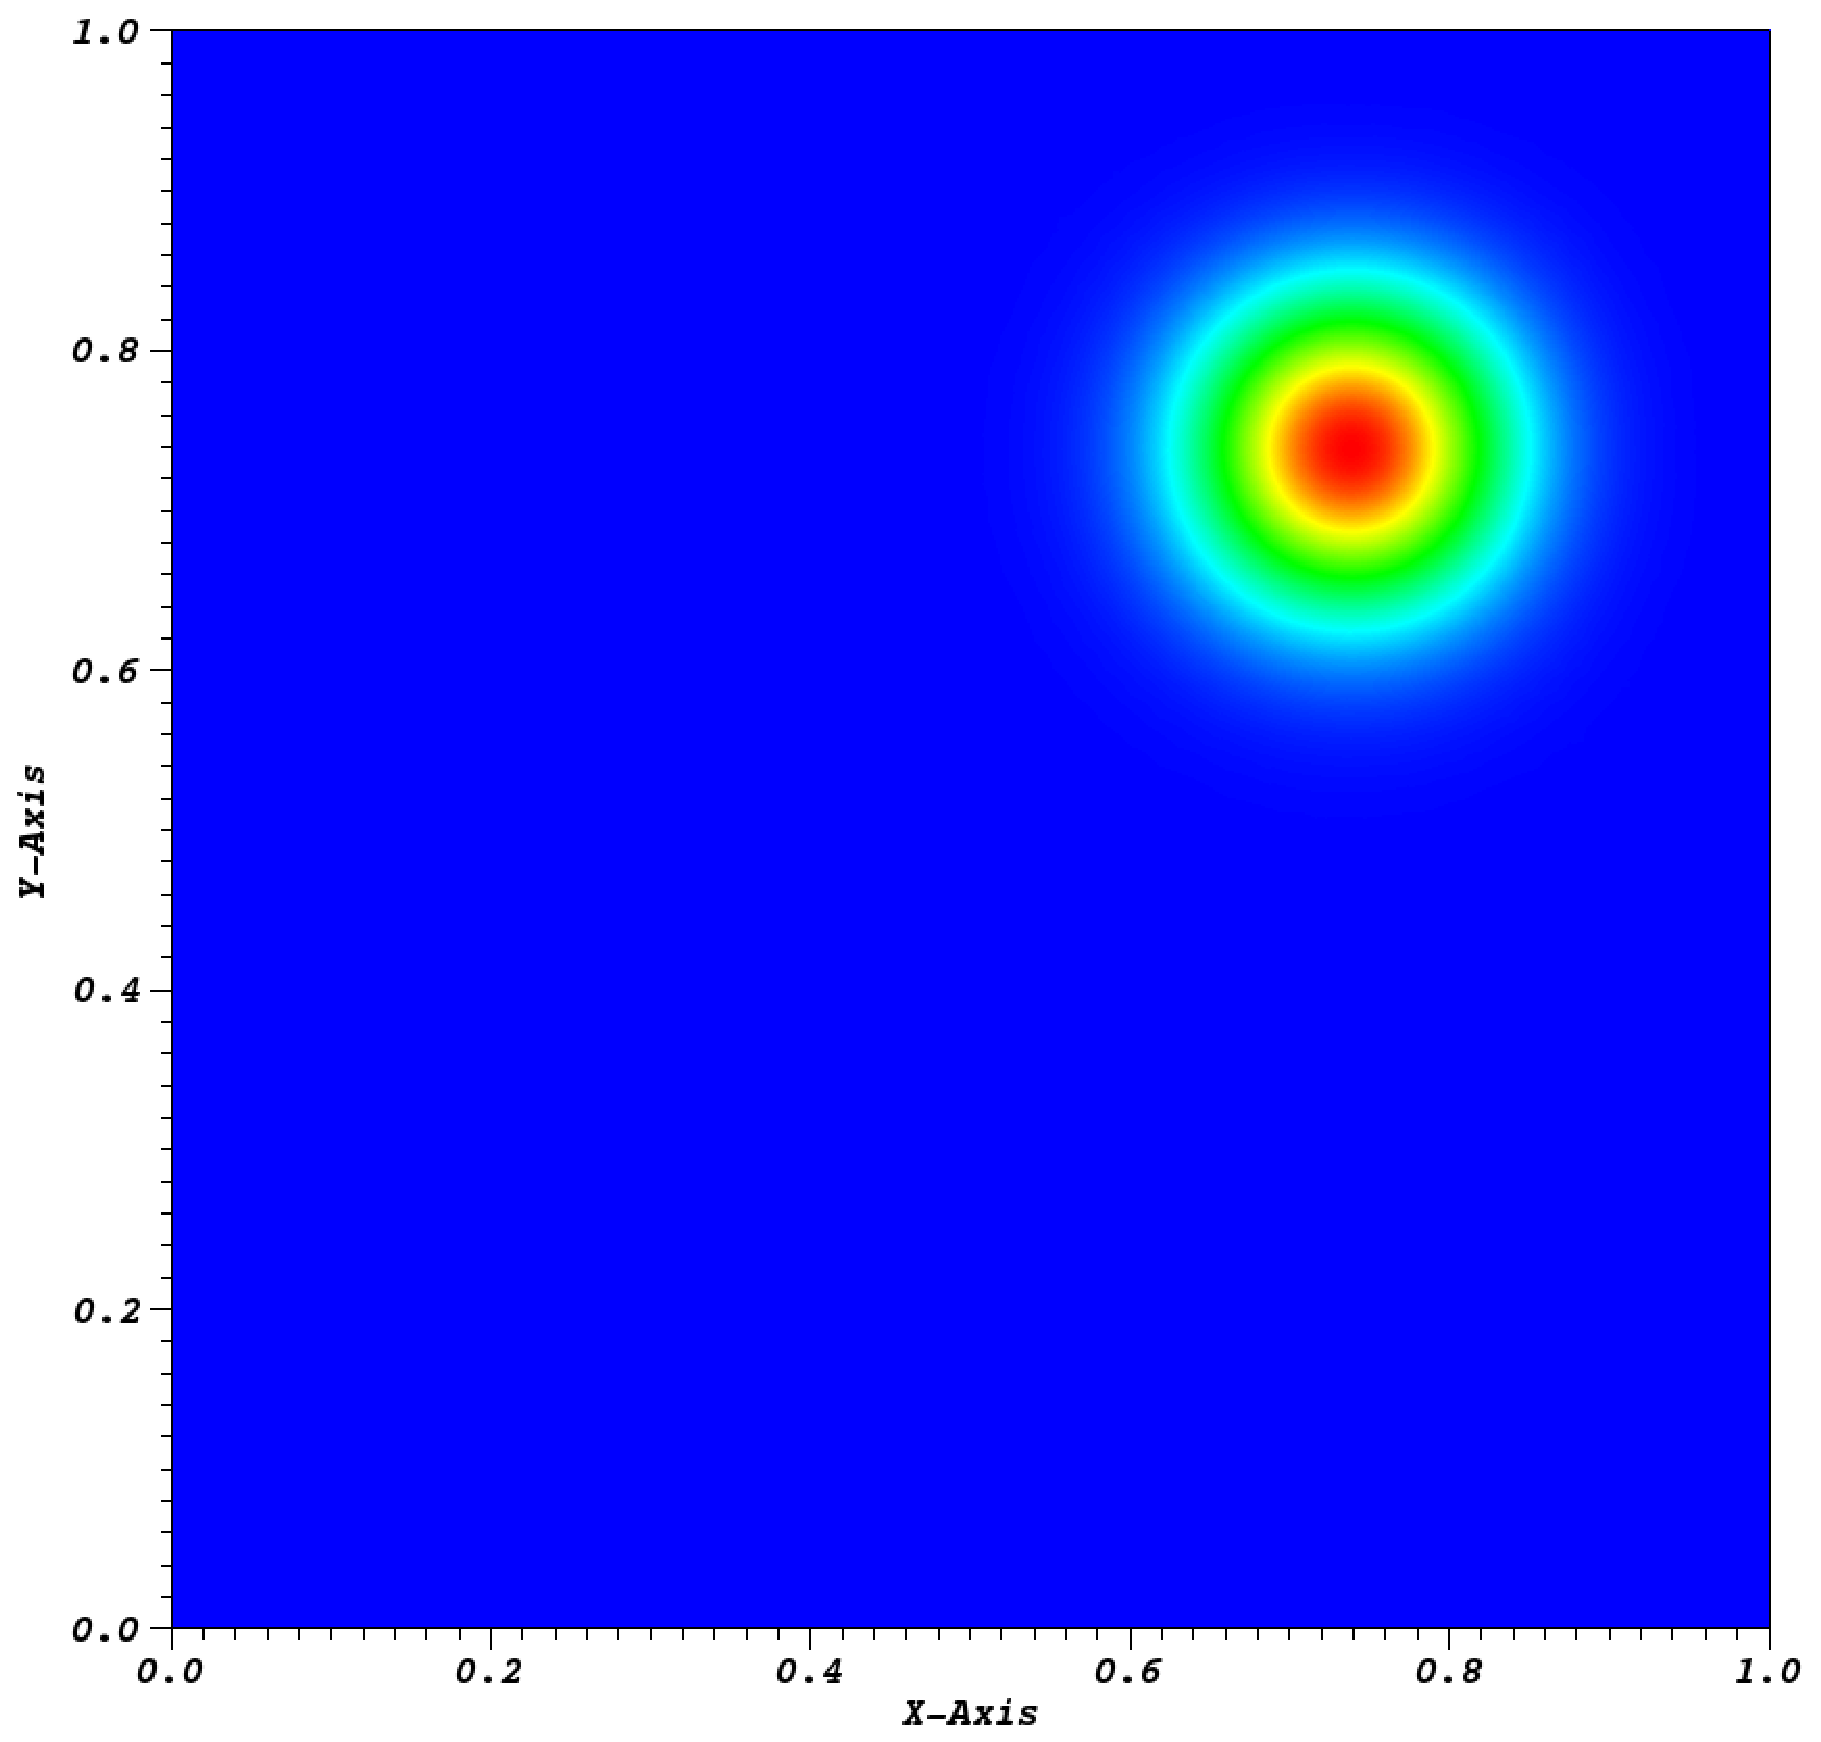
\includegraphics[width=0.70\columnwidth]{images/ME2_cart_Irr=1_tol=0.1_cyc08_sol.eps}
\end{columns}
}
\only<6>
{
\frametitle{Gaussian MMS Results - PWL}
\hspace*{1.25cm}
{}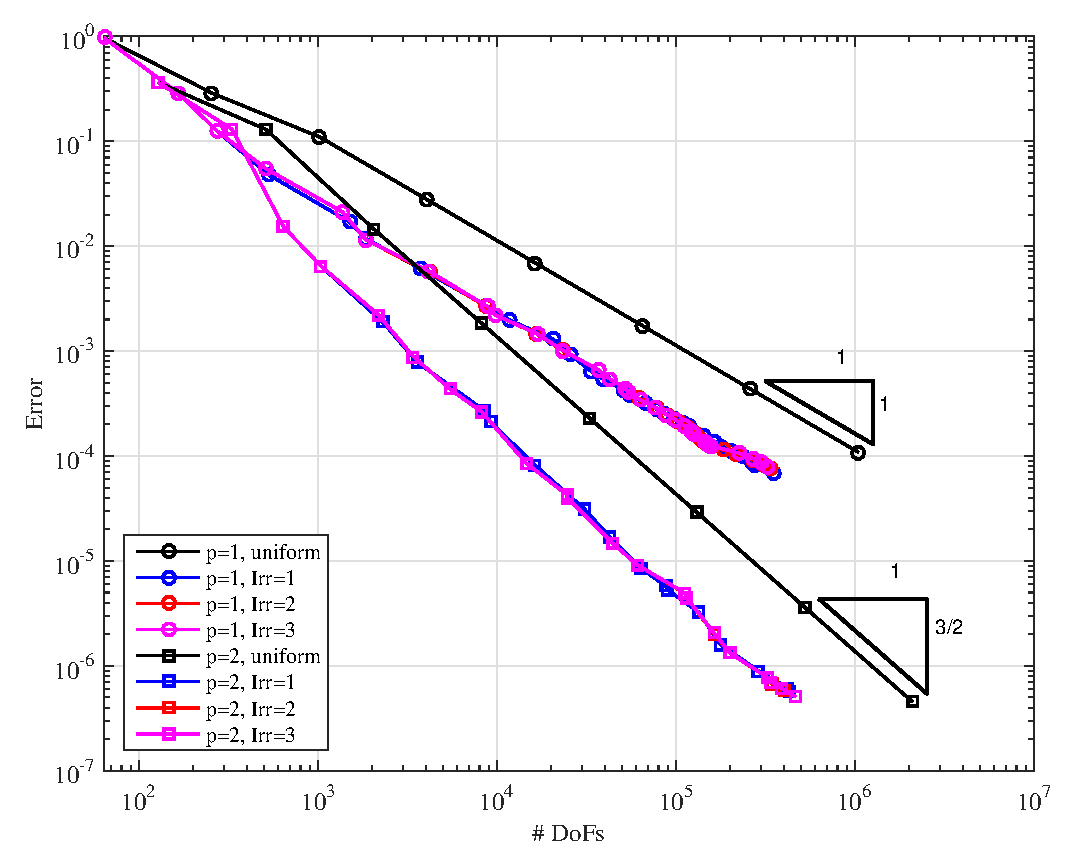
\includegraphics[width=0.75\columnwidth]{images/TransportMMS_Gauss2D_PWL_Err.eps}
}
\only<7>
{
\frametitle{Gaussian MMS Results - mean value}
\hspace*{1.25cm}
{}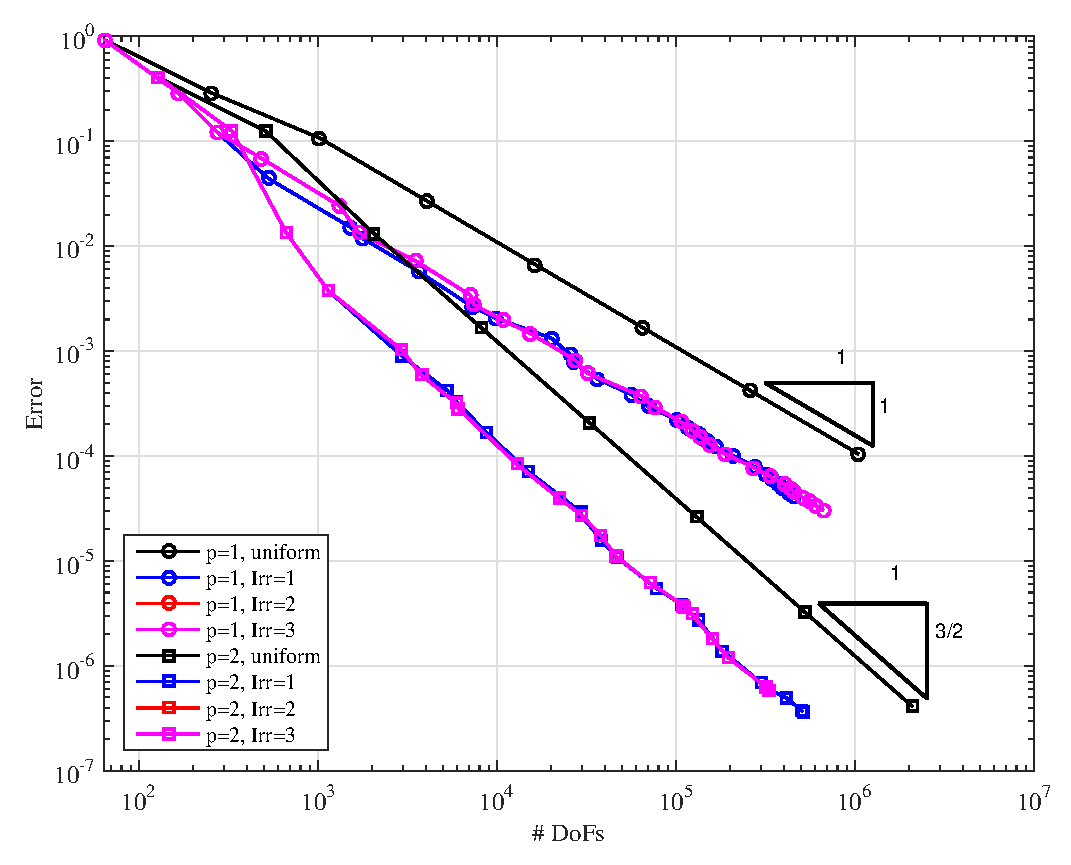
\includegraphics[width=0.75\columnwidth]{images/TransportMMS_Gauss2D_MV_Err.eps}
}
\only<8>
{
\frametitle{Gaussian MMS Results - maximum entropy}
\hspace*{1.25cm}
{}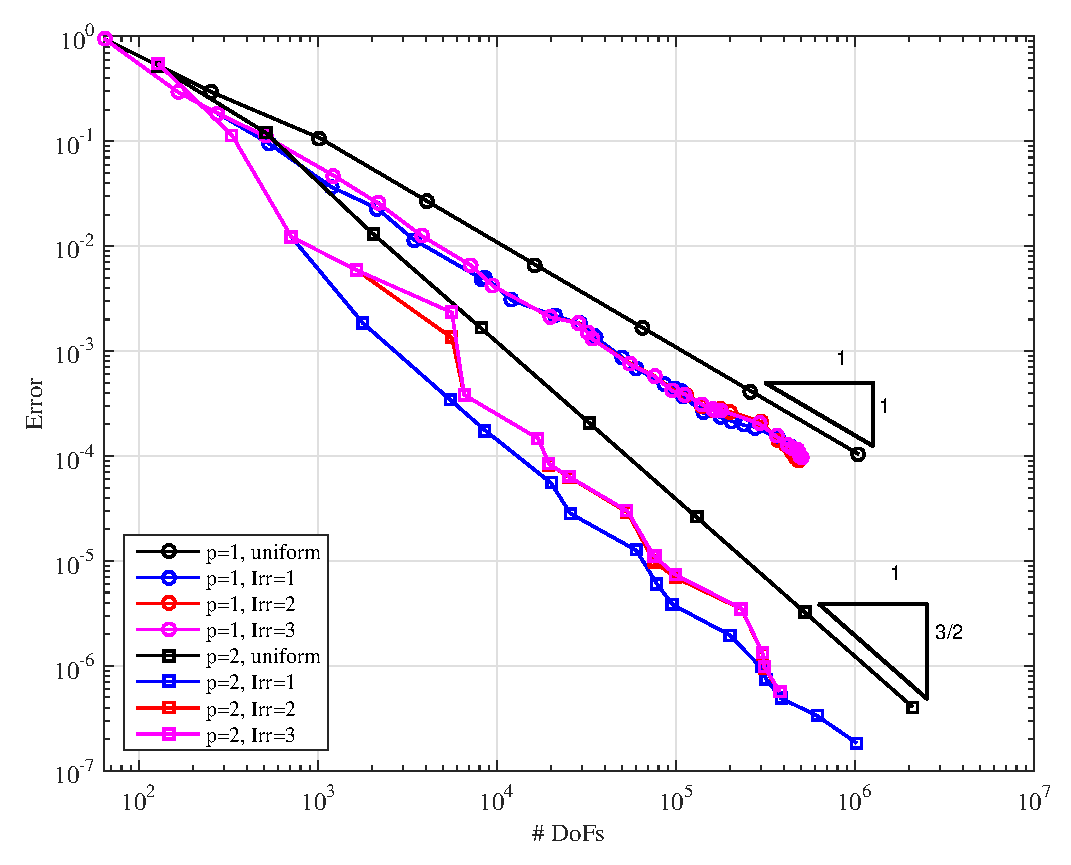
\includegraphics[width=0.75\columnwidth]{images/TransportMMS_Gauss2D_MAXENT_Err.eps}
}
\end{frame}
% --------------------------------------------
\begin{frame}[t]
\only<1>
{
\frametitle{Purely-Absorbing Material Problem}
\begin{block}{Problem Configuration}
\begin{enumerate}
\item Level-Symmetric $S_4$ quadrature
\end{enumerate}
\end{block}
\begin{block}{Geometry Configuration}
\begin{enumerate}
\item Unit square domain
\item Cartesian, Triangular, Polygonal, and Split-Polygonal Meshes
\end{enumerate}
\end{block}
}
\only<2>
{
\frametitle{Incident Flux Configuration}
\vspace{1cm}
\hspace*{2.75cm}
{}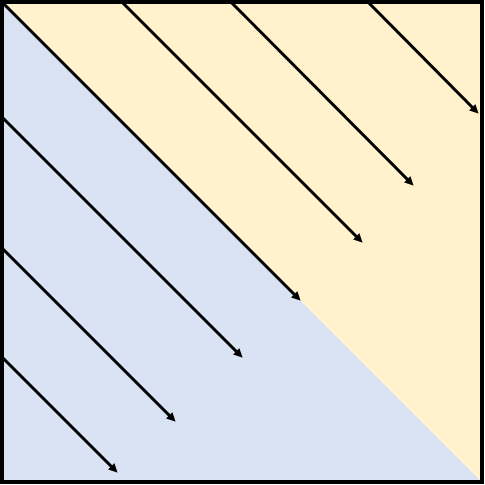
\includegraphics[width=0.45\textwidth]{images/PA_Shading.png}
}
\only<3>
{
\frametitle{Non-Aligned Meshes}
\vspace{0.75cm}
\hspace*{0.25cm}
{}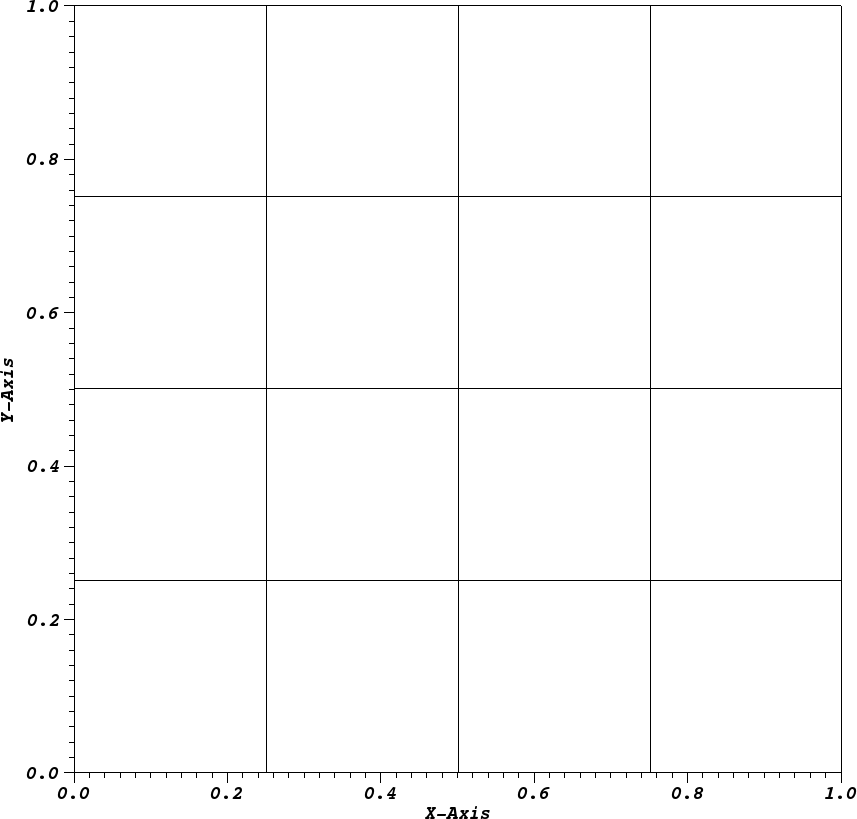
\includegraphics[width=0.475\textwidth]{images/PAMesh_Cart.png} 
{}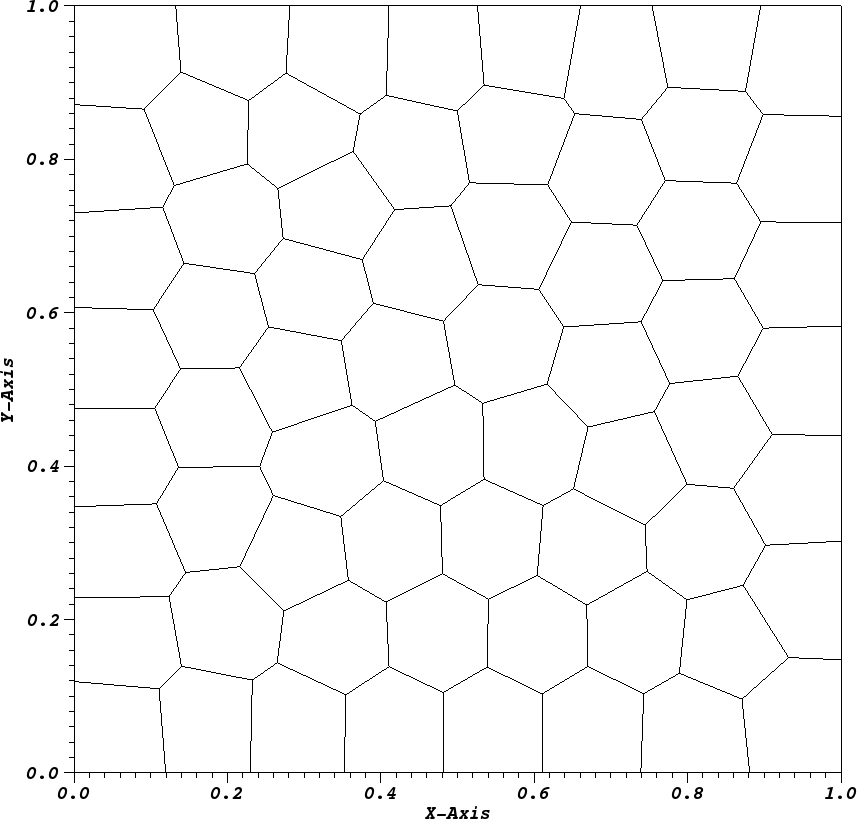
\includegraphics[width=0.475\textwidth]{images/PAMesh_Poly.png}
}
\only<4>
{
\frametitle{Aligned Meshes}
\vspace{0.75cm}
\hspace*{0.25cm}
{}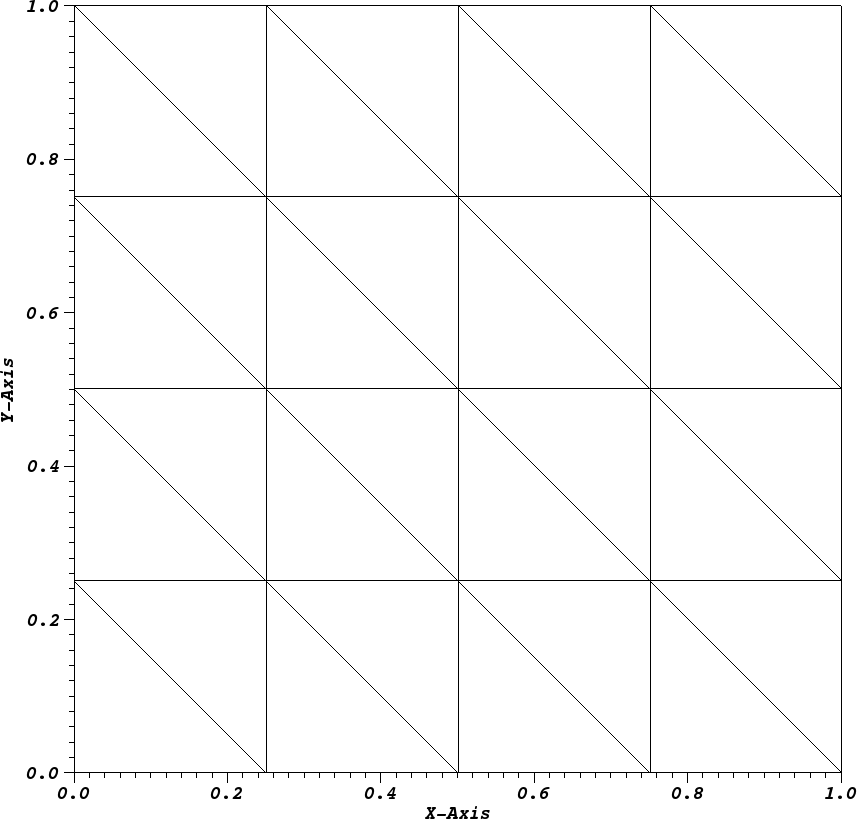
\includegraphics[width=0.475\textwidth]{images/PAMesh_Tri.png} 
{}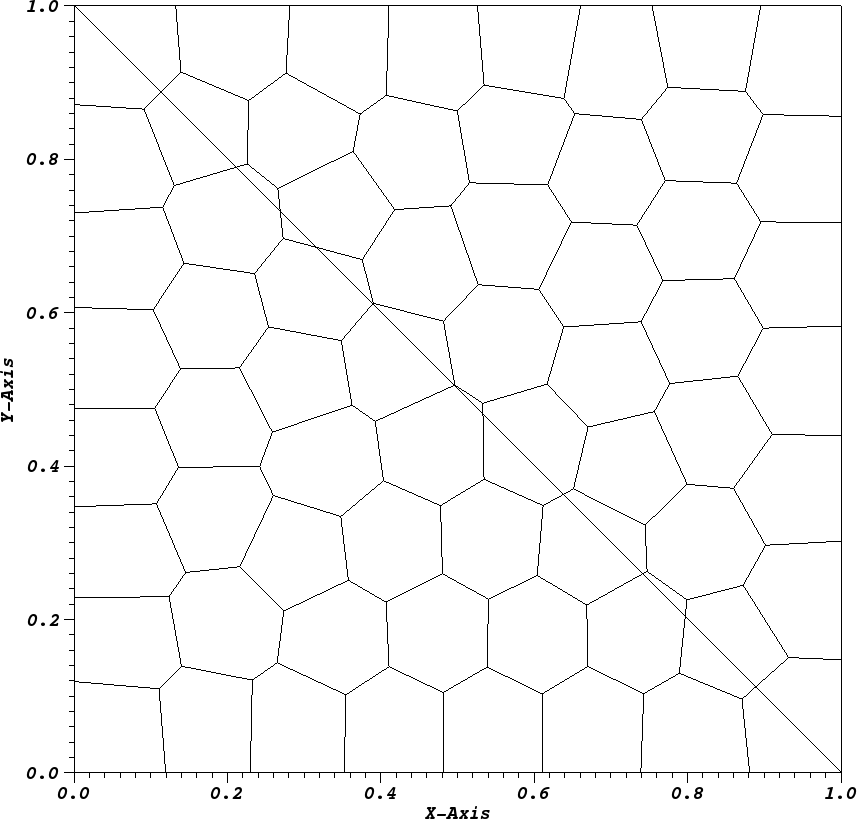
\includegraphics[width=0.475\textwidth]{images/PAMesh_SplitPoly.png}
}
\only<5>
{
\frametitle{Left-Face Incidence Solutions}
\vspace{0.75cm}
\hspace*{0.25cm}
{}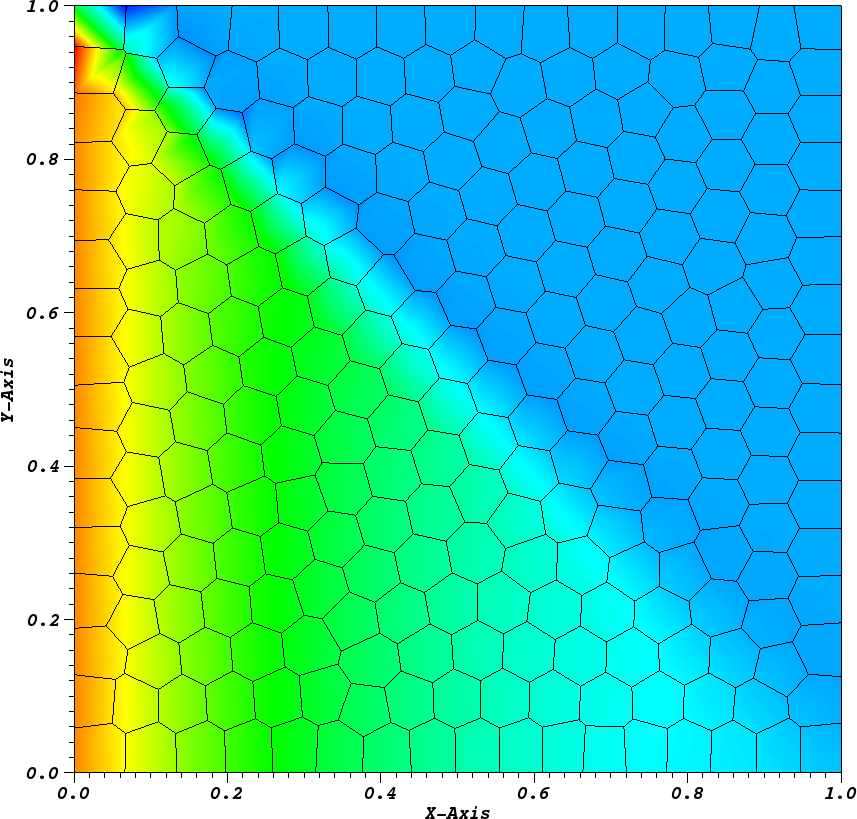
\includegraphics[width=0.475\textwidth]{images/PALeftSol_Poly.png} 
{}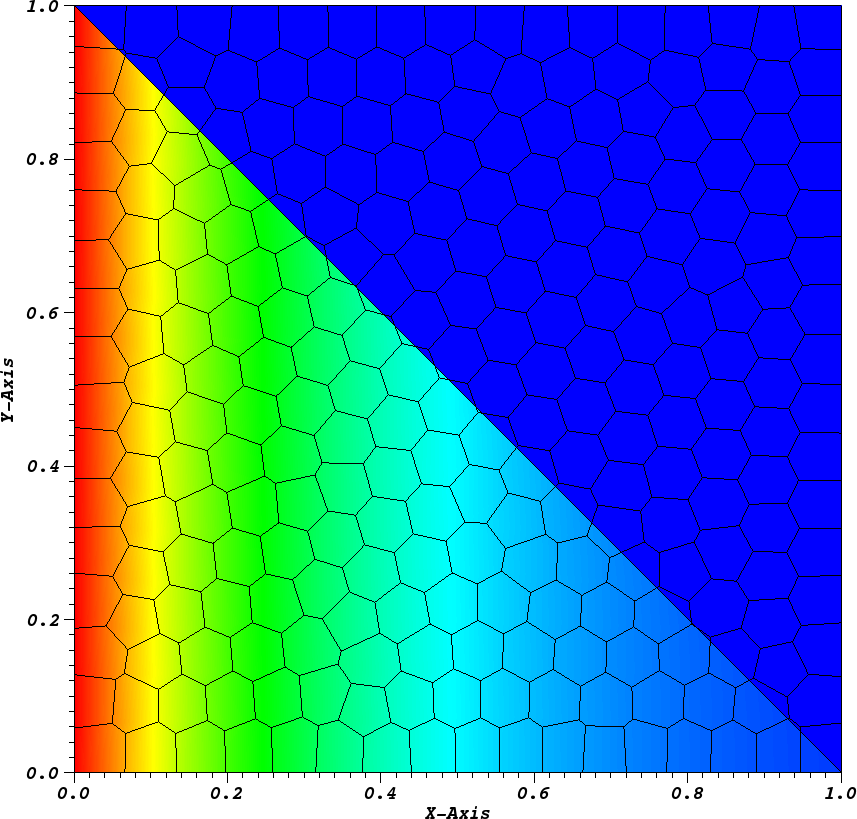
\includegraphics[width=0.475\textwidth]{images/PALeftSol_SplitPoly.png}
}
\only<6>
{
\frametitle{Left-Face and Top-Face Incidence Solutions}
\vspace{0.75cm}
\hspace*{0.25cm}
{}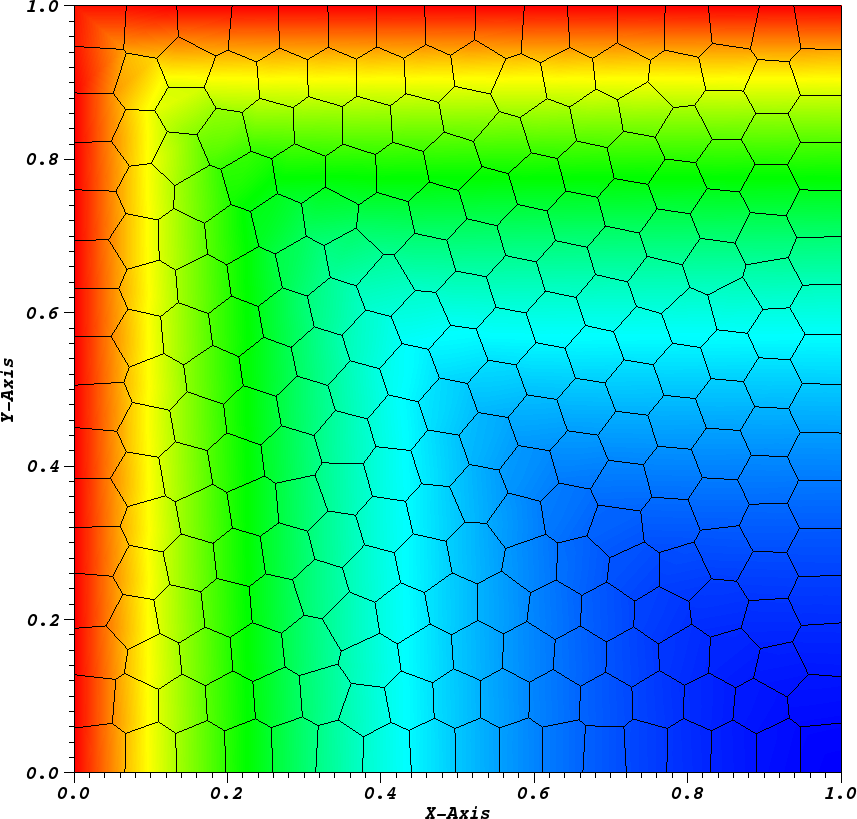
\includegraphics[width=0.475\textwidth]{images/PALeftTopSol_Poly.png} 
{}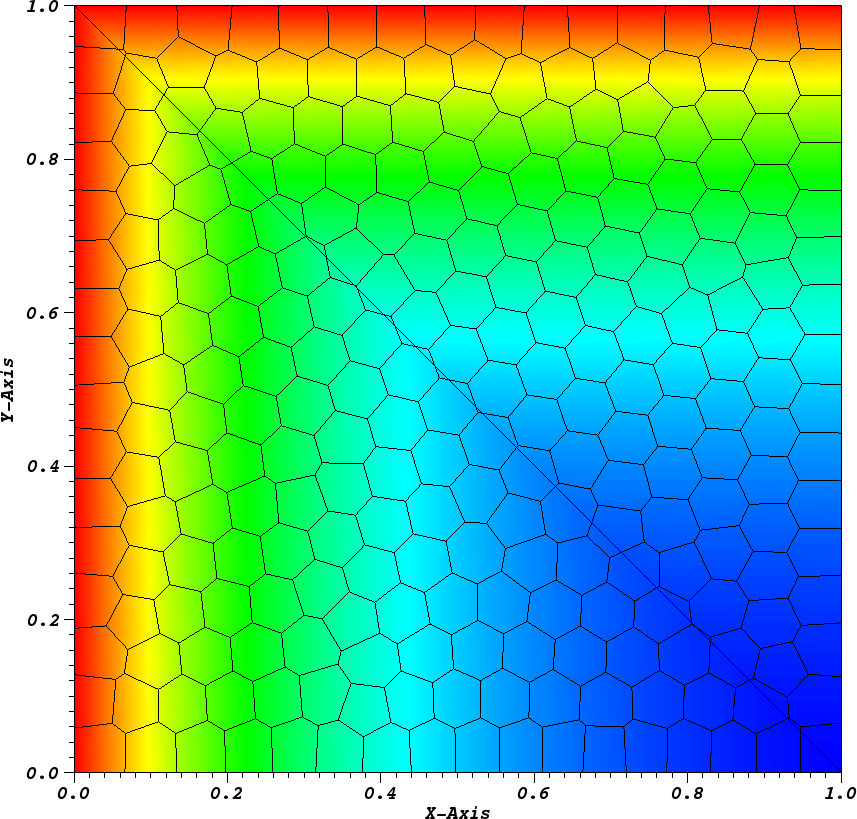
\includegraphics[width=0.475\textwidth]{images/PALeftTopSol_SplitPoly.png}
}
\only<7>
{
\frametitle{convergence rate plots go here...}
}
\end{frame}
% --------------------------------------------
%%%%%%%%%%%%%%%%%%%%%%%%%%%%%%%%%%%%%%%%%%%%%%%%%%%%%%%%%%%%%%%%%%%%%%%%%%%%%%%%%%%%%%%%%%%%%%
%%%%%%%%%%%%%%%%%%%%%%%%%%%%%%%%%%%%%%%%%%%%%%%%%%%%%%%%%%%%%%%%%%%%%%%%%%%%%%%%%%%%%%%%%%%%%%
\typeout{***********************************************************************************}
\typeout{MIP Section}
%%%%%%%%%%%%%%%%%%%%%%%%%%%%%%%%%%%%%%%%%%%%%%%%%%%%%%%%%%%%%%%%%%%%%%%%%%%%%%%%%%%%%%%%%%%%%%
% MIP SECTION
\section[MIP Form]{DFEM Discretization of the Diffusion Equation}
%%%%%%%%%%%%%%%%%%%
\subsection{}
%%%%%%%%%%%%%%%%%%%
% --------------------------------------------
\begin{frame}[t]\frametitle{Synthetic Acceleration}
\begin{block}{Transport sweep and iteration error}{\small
\begin{columns}
\column{0.60\textwidth}
\begin{equation*}
\begin{aligned}
{\bf L} \psi^{\tcr{(\ell+1/2)}} &= {\bf M\Sigma} \phi^{\tcb{(\ell)}} +{\bf Q} \\ \vspace{1mm}
{\bf L} \delta \psi^{\tcr{(\ell+1/2)}} &= {\bf M\Sigma} \delta \phi^{\tcr{(\ell+1/2)}} + \underbrace{{\bf M\Sigma} (\phi^{\tcr{(\ell+1/2)}}-\phi^{\tcb{(\ell)}})}_{{\bf R}^{\tcr{(\ell+1/2)}}} 
\end{aligned}
\end{equation*}
\column{0.40\textwidth}
\begin{equation*}
\begin{aligned}
\delta \psi^{\tcr{(\ell+1/2)}} &\equiv \psi - \psi^{\tcr{(\ell+1/2)}} \\
\delta \phi^{\tcr{(\ell+1/2)}} &\equiv {\bf D} \delta \psi^{\tcr{(\ell+1/2)}}
\end{aligned}
\end{equation*}
\end{columns}
}
\end{block}
\vspace{-1.5mm}
\begin{block}{Error approximation and update}{\small
If we could exactly solve for the error, then the solution could be obtained immediately:
\begin{equation*}
\phi^{(\ell+1)} = \phi^{\tcr{(\ell+1/2)}} + \delta \phi^{\tcr{(\ell+1/2)}}
\end{equation*}
However, this is just as difficult as the original transport problem. Instead, we estimate the error using low-order operators:
\begin{equation*}
\tilde{{\bf A}} \delta \phi^{\tcr{(\ell+1/2)}} = \tilde{{\bf R}}^{\tcr{(\ell+1/2)}}
\end{equation*}
$\tilde{{\bf A}}$ is a low-order diffusion operator.
}
\end{block}
\end{frame}
% --------------------------------------------
\begin{frame}[t]\frametitle{Various DSA Implementations}
\begin{block}{Historical DSA Work}
\begin{itemize}
	\item Kopp \& Lebedev - independently proposed method
	\item Gelbard and Hageman (G\&B) - efficient convergence on fine meshes
	\item Reed - showed that G\&B diverged for coarse meshes
	\item Alcouffe - consistency yields efficiency and robustness
\end{itemize}
\end{block}
\onslide<2->{
\begin{block}{Fully-consistent DSA schemes}
\begin{itemize}
	\item Larsen fully-consistent four step
	\item Fully-consistent DSA (FCDSA)
\end{itemize}
\end{block}
\begin{block}{Partially-consistent DSA schemes}
\begin{itemize}
	\item Modified four step (M4S)
	\item Waering-Larsen-Adams (WLA)
	\item Modified Interior Penalty DSA (MIP)
\end{itemize}
\end{block}
}
\end{frame}
% --------------------------------------------
%%%%%%%%%%%%%%%%%%%
\subsection{Symmetric Interior Penalty Method}
%%%%%%%%%%%%%%%%%%%
%---------------------------
\begin{frame}[t]\frametitle{Symmetric Interior Penalty (SIP) Form [1]}
\begin{block}{Bilinear Form}{\small
\begin{equation*}
\begin{aligned}
a( \Phi, b)  &= \Big<  D \vec{\nabla}  \Phi , \vec{\nabla} b  \Big>_{\mathcal{D}} + \Big<  \sigma   \Phi ,  b  \Big>_{\mathcal{D}}    \\
&+  \tcr{\Big\{ \kappa_e^{SIP} [\![   \Phi ]\!] , [\![  b ]\!]\Big\}_{E_h^i}} - \tcr{\Big\{  [\![   \Phi ]\!] , \{\!\{  D \partial_n b \}\!\}\Big\}_{E_h^i}} -\tcr{\Big\{ \{\!\{  D \partial_n  \Phi \}\!\} , [\![ b ]\!]\Big\}_{E_h^i}} \\
&+ \tcb{\Big\{ \kappa_e^{SIP}   \Phi ,   b \Big\}_{\partial \mathcal{D}^d}} - \tcb{\Big\{   \Phi  ,  D \partial_n b \Big\}_{\partial \mathcal{D}^d}} - \tcb{\Big\{   D \partial_n  \Phi ,   b \Big\}_{\partial \mathcal{D}^d}}  +  \tcb{\frac{1}{2} \Big\{    \Phi ,   b \Big\}_{\partial \mathcal{D}^r}}
\end{aligned}
\end{equation*} }
\end{block}
\begin{block}{Linear Form}{\small
\begin{align*}
\ell (b) = \Big<  q, b  \Big>_{\mathcal{D}}  - \tcb{\Big\{   J_{0}, b  \Big\}_{\partial \mathcal{D}^n}} +  \tcb{2 \Big\{   J_{inc}, b  \Big\}_{\partial \mathcal{D}^r}} \\ + \tcb{\Big\{ \kappa_e^{SIP}   \Phi_0 ,   b \Big\}_{\partial \mathcal{D}^d}} - \tcb{\Big\{   \Phi_0  ,  D \partial_n b \Big\}_{\partial \mathcal{D}^d} }
\end{align*} }
\end{block}
\begin{block}{}{\footnotesize
[1] D.N. Arnold. ``An interior penalty finite element method with discontinuous elements.'' {\em SIAM J. Numer. Anal.}, 19:742-760, (1982).
}\end{block}
\end{frame}
%---------------------------
\begin{frame}[t]\frametitle{SIP Penalty Coefficient}
\begin{block}{}{
	\begin{equation*}
		\kappa_e^{SIP} \equiv 
		\begin{cases}
		\frac{C_B}{2} \left(  \frac{D^+}{h^+} + \frac{D^-}{h^-}  \right) & , e \in E_h^i \\
		C_B \frac{D^-}{h^-}  & , e \in \partial \mathcal{D}
		\end{cases}
	\end{equation*}}
	\begin{equation*}
		C_B = c p (p+1)
	\end{equation*}
\end{block}
\begin{block}{}
$c$ - user defined constant ($c \geq 1$) \\
$p$ - polynomial order of the finite element basis ($1,2,3,...$) \\
$D^{(+/-)}$ - diffusion coefficient defined on the positive/negative side of a face\\
$h^{(+/-)}$ - orthogonal projection defined on the positive/negative side of a face
\end{block}
\begin{block}{}
	\begin{equation*}
		u^{\pm} = \lim_{s \rightarrow 0^{\pm}} u ({\bf r} + s {\bf n})
	\end{equation*}
\end{block}
\end{frame}
%---------------------------
%%%%%%%%%%%%%%%%%%%
\subsection{Modified Interior Penalty Method}
%%%%%%%%%%%%%%%%%%%
%---------------------------
\begin{frame}[t]\frametitle{Modified Interior Penalty (MIP) Form}

Recall the DSA equation:
\begin{equation*}
{\bf \tilde{A}} \tcr{\delta \phi}^{(\ell+1/2)} = \tilde{{\bf R}}^{(\ell+1/2)}
\end{equation*}

\begin{block}{Diffusion Form}{\footnotesize
\begin{gather*}
\Big<  D \vec{\nabla} \tcr{\delta \Phi} , \vec{\nabla} b  \Big>_{\mathcal{D}} 
+ \Big<  \sigma \tcr{\delta  \Phi} ,  b  \Big>_{\mathcal{D}}    \\
+ \Big\{ \kappa_e^{MIP} [\![ \tcr{\delta  \Phi} ]\!] , [\![  b ]\!]\Big\}_{E_h^i} 
- \Big\{  [\![  \tcr{\delta \Phi} ]\!] , \{\!\{  D \partial_n b \}\!\}\Big\}_{E_h^i} 
- \Big\{ \{\!\{  D \partial_n \tcr{\delta \Phi} \}\!\} , [\![ b ]\!]\Big\}_{E_h^i} \\
+ \Big\{ \kappa_e^{MIP} \tcr{\delta \Phi} ,   b \Big\}_{\partial \mathcal{D}^{vac}} -  \frac{1}{2} \Big\{  \tcr{\delta \Phi}  ,  D \partial_n b \Big\}_{\partial \mathcal{D}^{vac}} -  \frac{1}{2} \Big\{   D \partial_n \tcr{\delta \Phi} ,   b \Big\}_{\partial \mathcal{D}^{vac}}  \\
 = \Big<  R , b  \Big>_{\mathcal{D}}  +  \Big\{  \tcr{\delta J_{inc}}, b  \Big\}_{\partial \mathcal{D}^{ref}}
\end{gather*} }
\end{block}
	\begin{block}{MIP Penalty Term}{\footnotesize
		\begin{align*}
			\kappa_e^{MIP} = \max(\frac{1}{4},  \kappa_e^{SIP})
		\end{align*} }
	\end{block}
\end{frame}
%---------------------------
%%%%%%%%%%%%%%%%%%%
\subsection{Results}
%%%%%%%%%%%%%%%%%%%
% --------------------------------------------
\begin{frame}[t]
\only<1>
{
\frametitle{\small 2D Unit Square Fourier Results - linear (left) and quadratic (right) Wachspress}
\vspace{1cm}
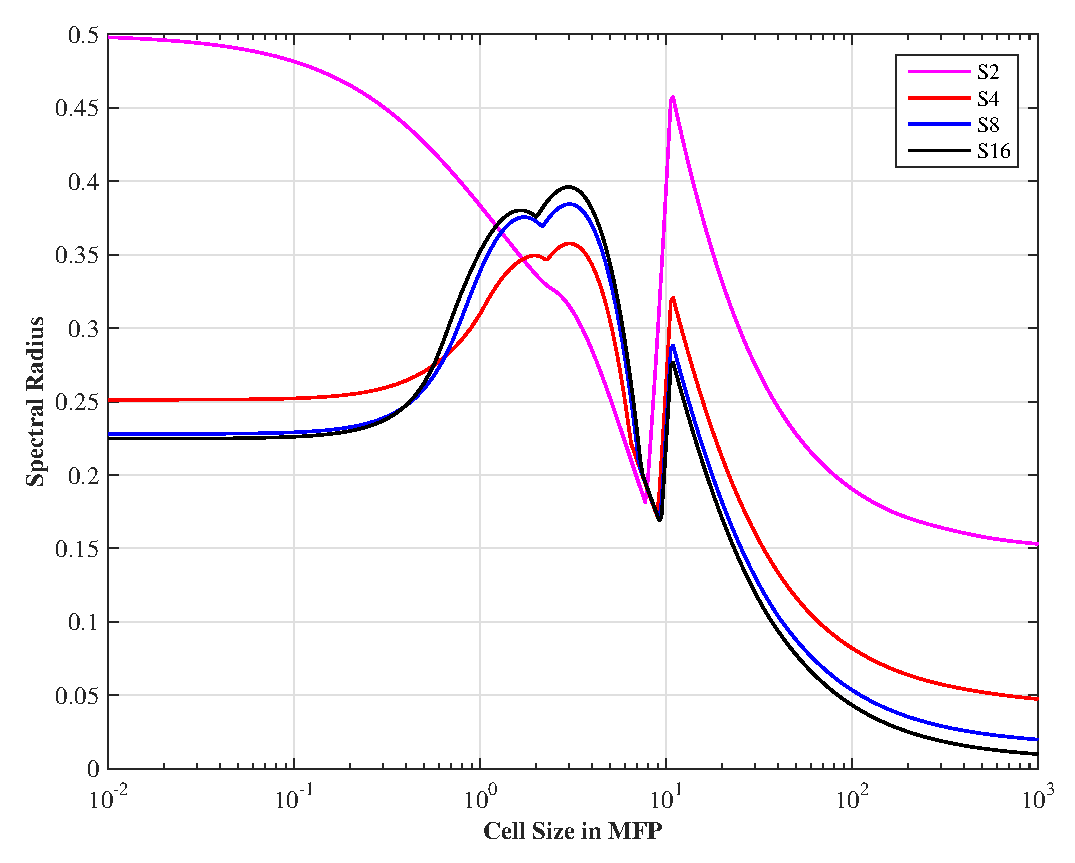
\includegraphics[width=0.495\textwidth]{images/SI_MIP_quad_C=4_UWACHSPRESS1_LS.eps}
\includegraphics[width=0.495\textwidth]{images/SI_MIP_quad_C=4_UWACHSPRESS2_LS.eps}
}
\only<2>
{
\frametitle{\small 2D Unit Square Fourier Results - linear (left) and quadratic (right) PWL}
\vspace{1cm}
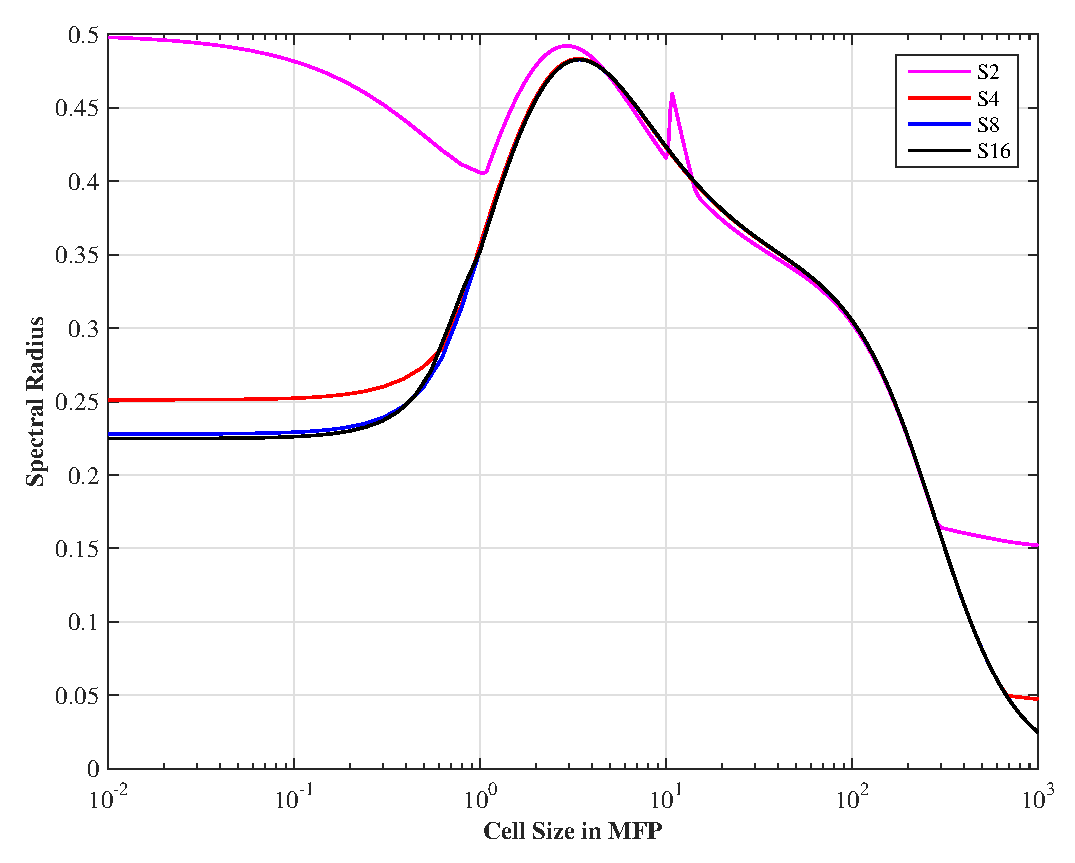
\includegraphics[width=0.495\textwidth]{images/SI_MIP_quad_C=4_PWLD1_LS.eps}
\includegraphics[width=0.495\textwidth]{images/SI_MIP_quad_C=4_UPWLD2_LS.eps}
}
\only<3>
{
\frametitle{\small 2D Unit Square Fourier Results - linear (left) and quadratic (right) Mean Value}
\vspace{1cm}
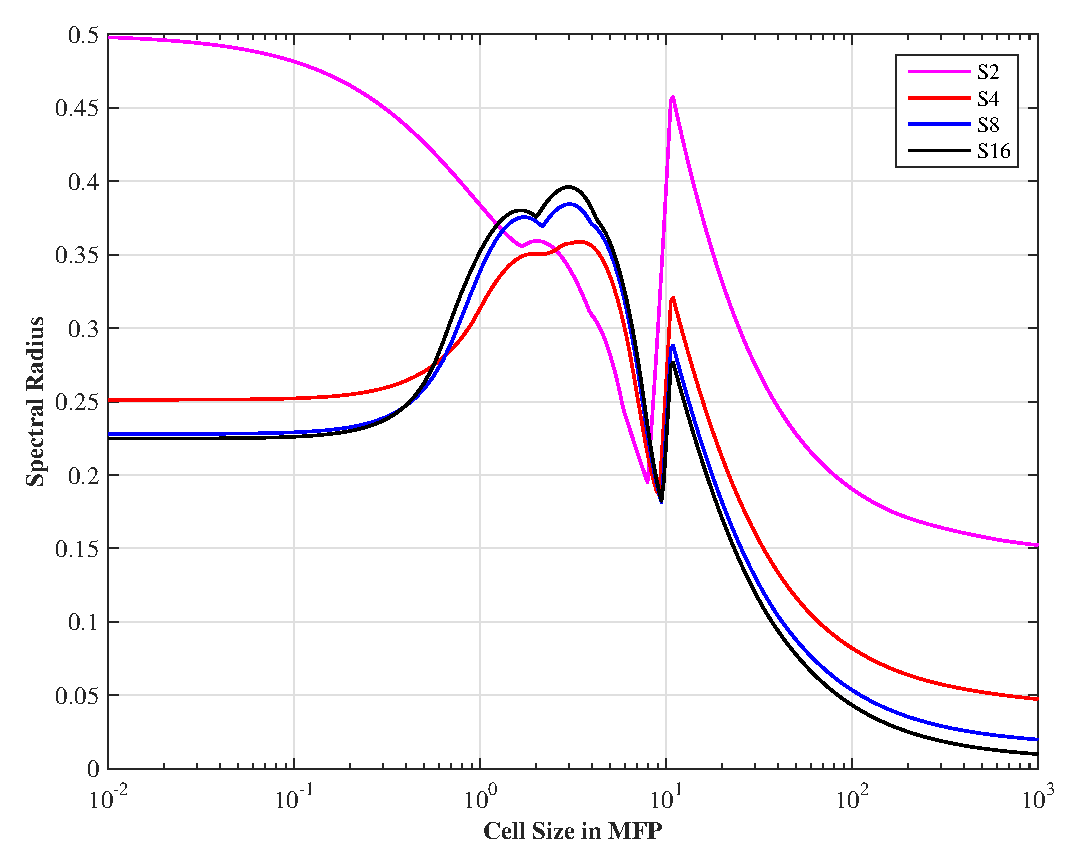
\includegraphics[width=0.495\textwidth]{images/SI_MIP_quad_C=4_UMV1_LS.eps}
\includegraphics[width=0.495\textwidth]{images/SI_MIP_quad_C=4_UMV2_LS.eps}
}
\only<4>
{
\frametitle{\small 2D Unit Square Fourier Results - linear (left) and quadratic (right) Maximum Entropy}
\vspace{1cm}
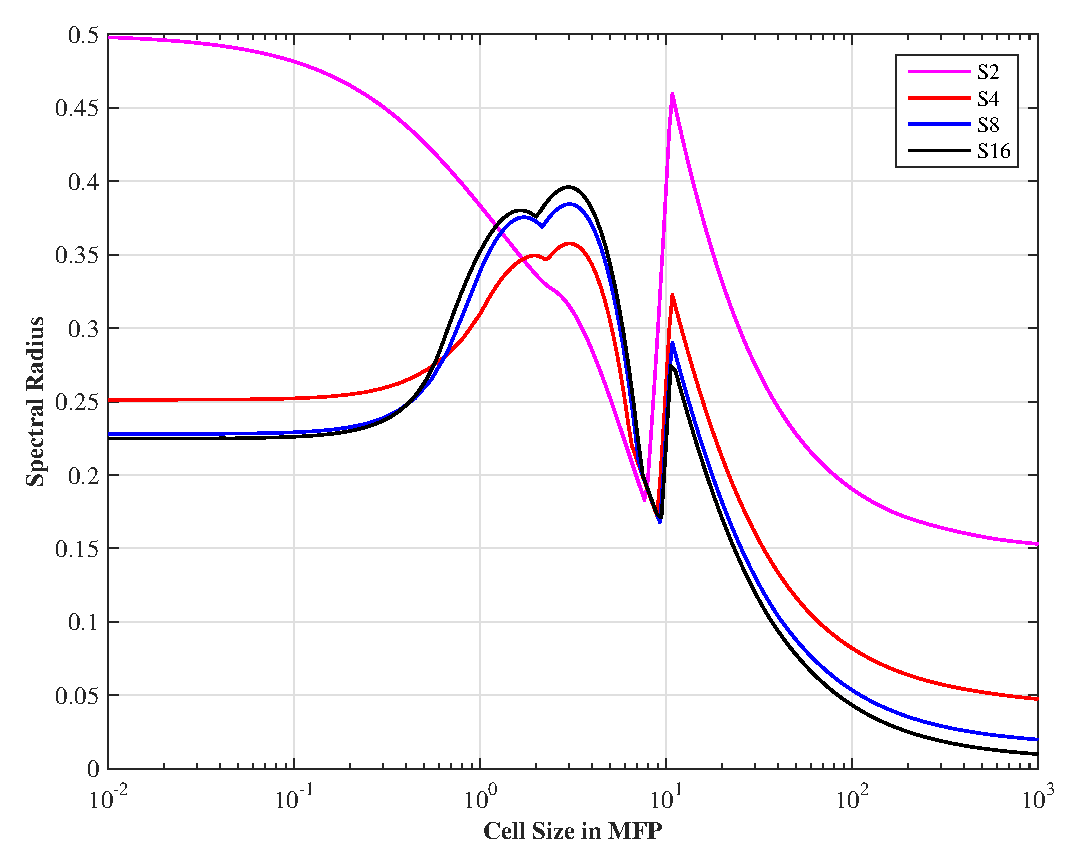
\includegraphics[width=0.495\textwidth]{images/SI_MIP_quad_C=4_MAXENT1_LS.eps}
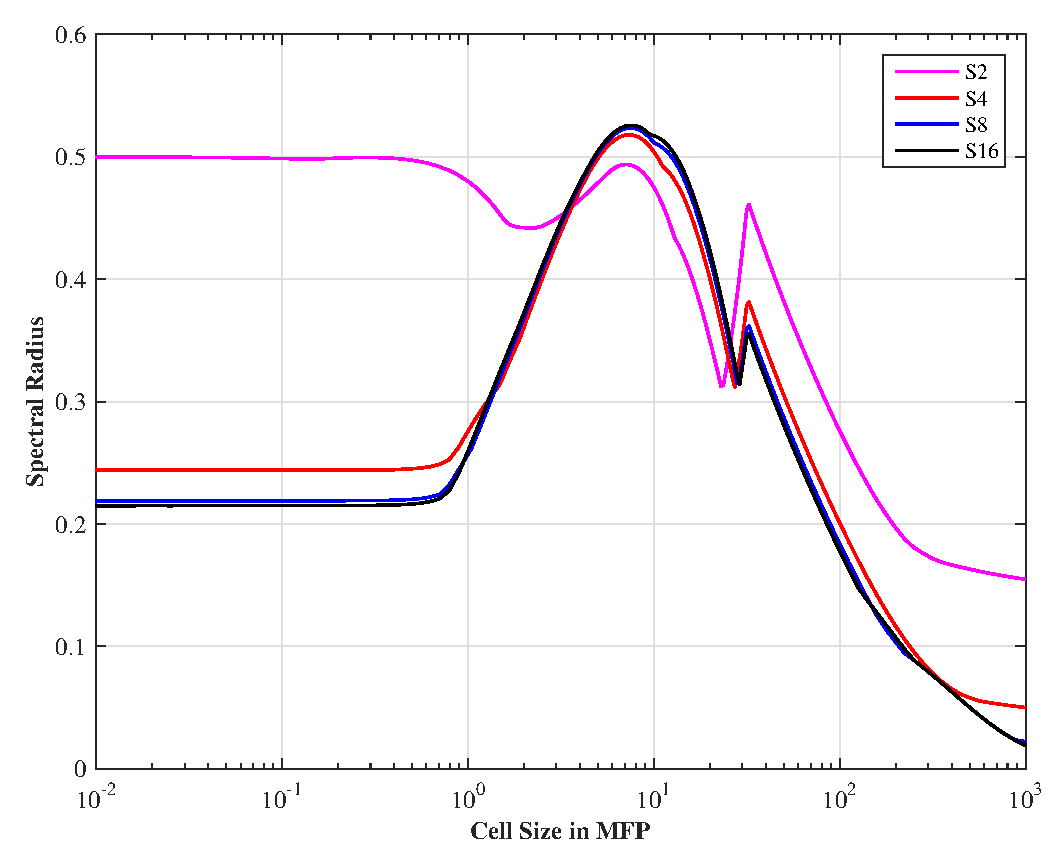
\includegraphics[width=0.495\textwidth]{images/SI_MIP_quad_C=4_UMAXENT2_LS.eps}
}
\end{frame}
% --------------------------------------------
\begin{frame}[t]\frametitle{DSA and AMR on Polygonal Grids}

\end{frame}
% --------------------------------------------
\begin{frame}[t]\frametitle{Analytical/Numerical 3D Results}

\end{frame}
% --------------------------------------------
\begin{frame}[t]\frametitle{MIP Scaling Results}

\end{frame}
% --------------------------------------------
%%%%%%%%%%%%%%%%%%%%%%%%%%%%%%%%%%%%%%%%%%%%%%%%%%%%%%%%%%%%%%%%%%%%%%%%%%%%%%%%%%%%%%%%%%%%%%
%%%%%%%%%%%%%%%%%%%%%%%%%%%%%%%%%%%%%%%%%%%%%%%%%%%%%%%%%%%%%%%%%%%%%%%%%%%%%%%%%%%%%%%%%%%%%%
\typeout{***********************************************************************************}
\typeout{Upscatter Section}
%%%%%%%%%%%%%%%%%%%%%%%%%%%%%%%%%%%%%%%%%%%%%%%%%%%%%%%%%%%%%%%%%%%%%%%%%%%%%%%%%%%%%%%%%%%%%%
% UPSCATTERING SECTION
\section[Upscattering Acceleration]{Thermal Neutron Upscattering Acceleration}
%%%%%%%%%%%%%%%%%%%
\subsection{Overview of Methods}
%%%%%%%%%%%%%%%%%%%
% --------------------------------------------
\begin{frame}[t]\frametitle{Overview of Methods}

\end{frame}
% --------------------------------------------
%%%%%%%%%%%%%%%%%%%
\subsection{IM1 Results}
%%%%%%%%%%%%%%%%%%%
% --------------------------------------------
\begin{frame}[t]\frametitle{IM1 Problem}

\end{frame}
% --------------------------------------------
\begin{frame}[t]
\only<1>
{
\frametitle{IM1 Two-Grid Spectral Shapes}
\hspace*{1.1cm}
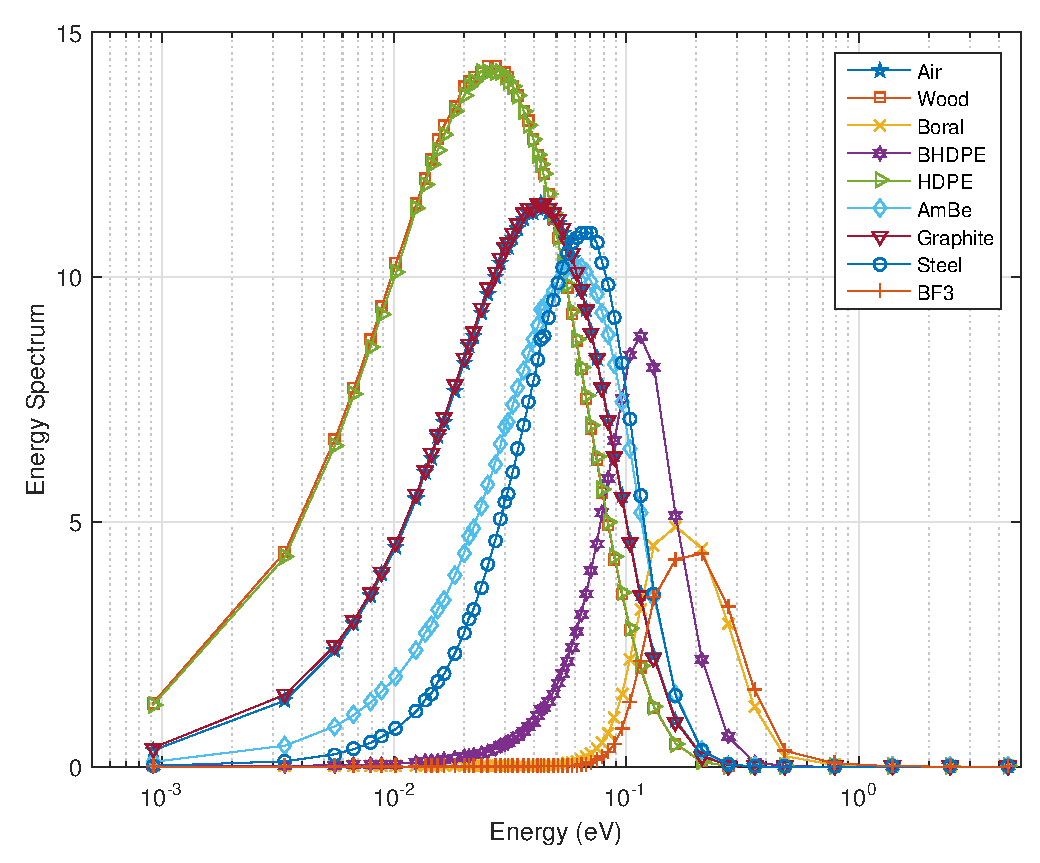
\includegraphics[width=0.75\textwidth]{images/IM1_EC_TG.eps}
}
\only<2>
{
\frametitle{IM1 Modified Two-Grid Spectral Shapes}
\hspace*{1.1cm}
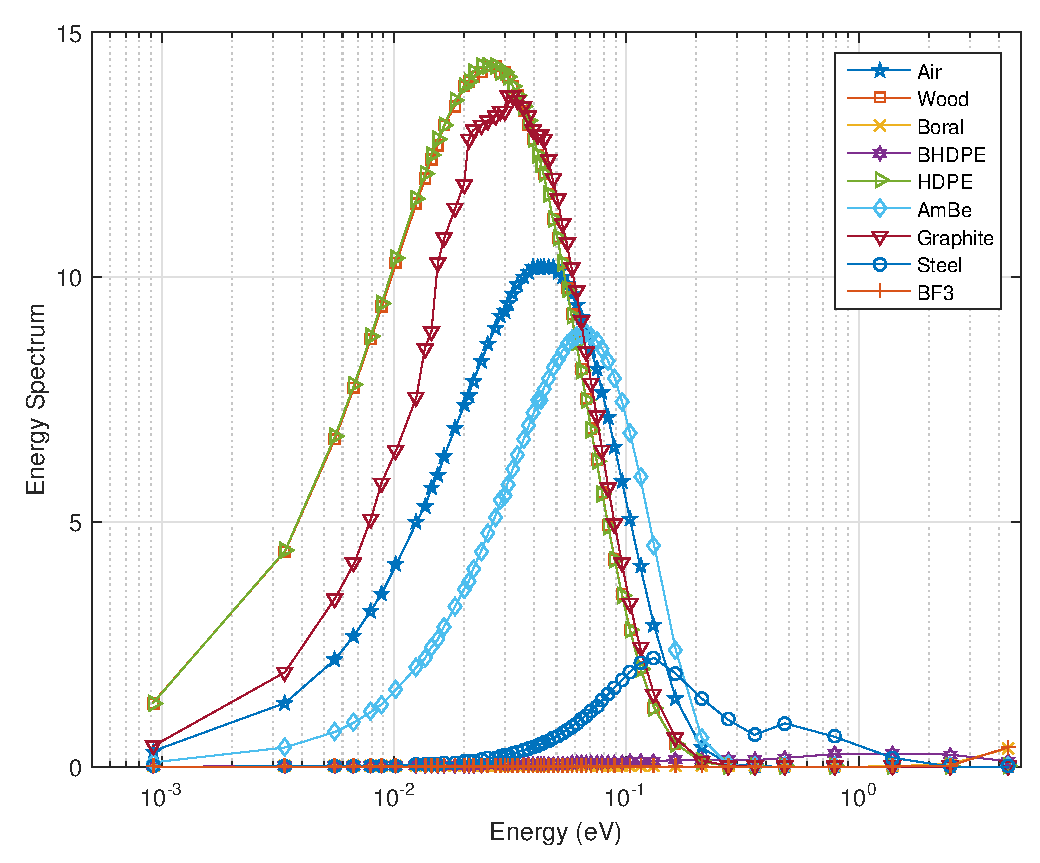
\includegraphics[width=0.75\textwidth]{images/IM1_EC_MTG.eps}
}
\only<3>
{
\frametitle{IM1 Multigroup Jacobi Acceleration Spectral Shapes}
\hspace*{1.1cm}
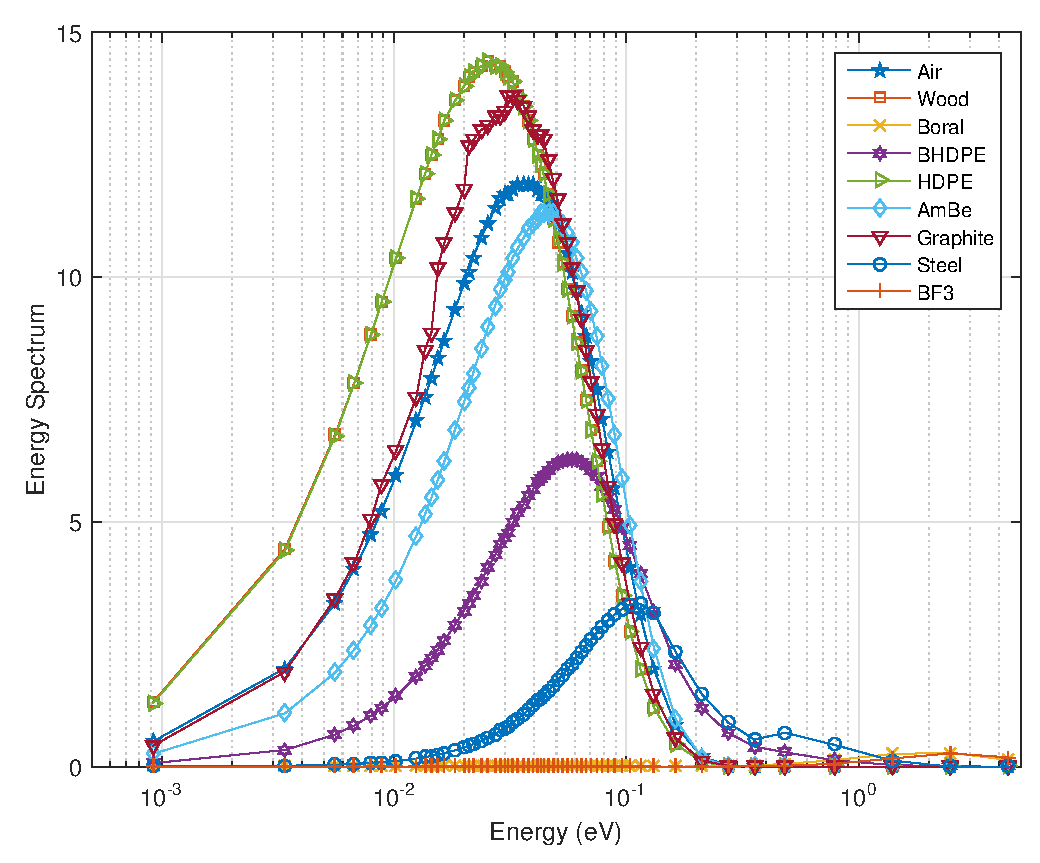
\includegraphics[width=0.75\textwidth]{images/IM1_EC_Rich.eps}
}
\only<4>
{
\frametitle{IM1 Multigroup Jacobi with Inner Acceleration Spectral Shapes}
\hspace*{1.1cm}
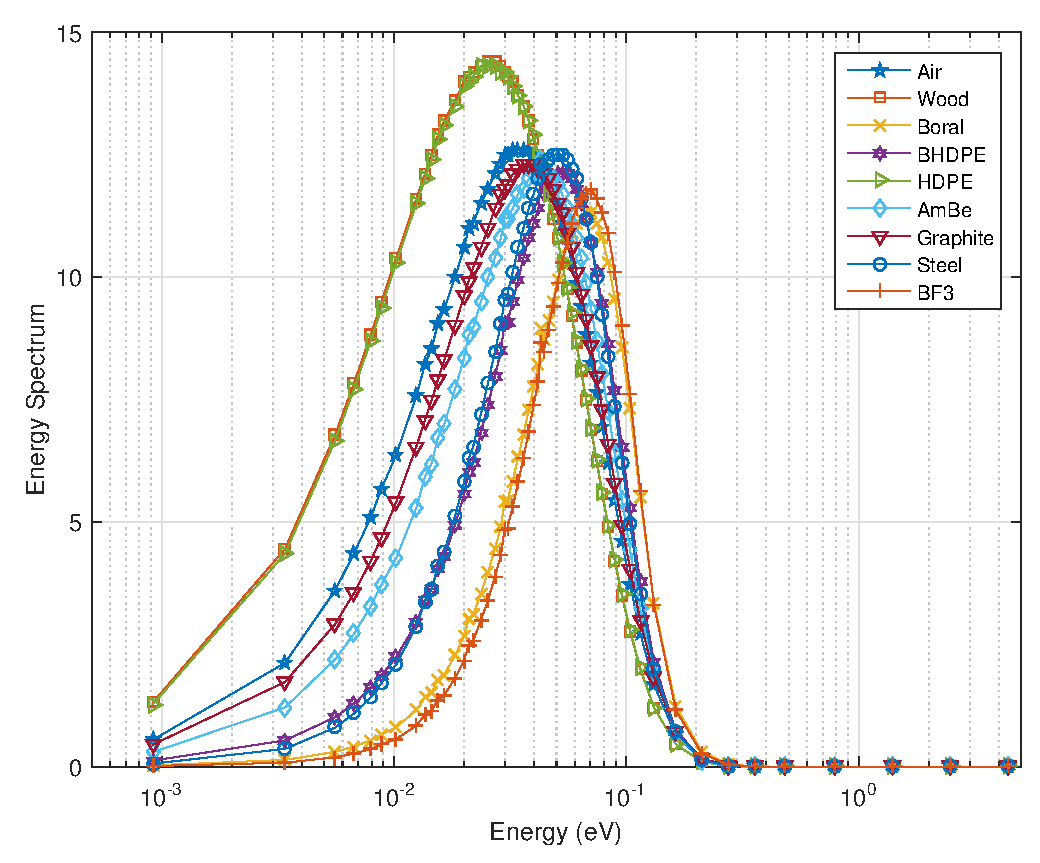
\includegraphics[width=0.75\textwidth]{images/IM1_EC_MJIA.eps}
}
\end{frame}
% --------------------------------------------
\begin{frame}[t]\frametitle{Infinite Medium Fourier Results}{\small
\vspace{0.85cm}
\begin{table}
\centering
\def\arraystretch{1.2}
\begin{tabular}{|c||c|c||c|c||c|c|c|}
\hline
Material  & U. TG & A. TG & U. MTG & A. MTG & U. MJA & A. MJA & A. MJIA \\ \hline
\tcr{Graphite} & \tcr{0.9883}&\tcb{0.4084}&\tcr{0.9993}&\tcr{0.9604}&\tcr{0.9993}&\tcr{0.9613}&\tcm{0.6462}\\
\tcr{HDPE} &\tcr{0.8916}&\tcb{0.4343}&\tcr{0.9918}&\tcr{0.7527}&\tcr{0.9943}&\tcr{0.8015}&\tcm{0.6631}\\
B-HDPE &0.0258&0.0177&0.1331&0.1221&0.1336&0.1223&0.0639 \\
Wood & 0.9820&0.2101&0.9840&0.3836&0.9915&0.5326&0.4684 \\
AmBe  &0.4835&0.2724&0.5646&0.5554&0.7068&0.5596&0.4947 \\
Steel  & 0.6989&0.5809&0.9243&0.9215&0.9255&0.9215&0.7547\\
Boral  & 0.0023&0.0016&0.0782&0.0602&0.0782&0.0602&0.0039 \\
BF3   & 0.0008&0.0006&0.0351&0.0266&0.0351&0.0266&0.0086 \\
Air     &0.7580&0.5282&0.8121&0.7828&0.8845&0.7896&0.7166\\
\hline
\end{tabular}
\end{table}
}\end{frame}
% --------------------------------------------
\begin{frame}[t]
\only<1>
{
\frametitle{\small Graphite Two-Grid Flat Mode Eigenvalues}
\hspace*{1.1cm}
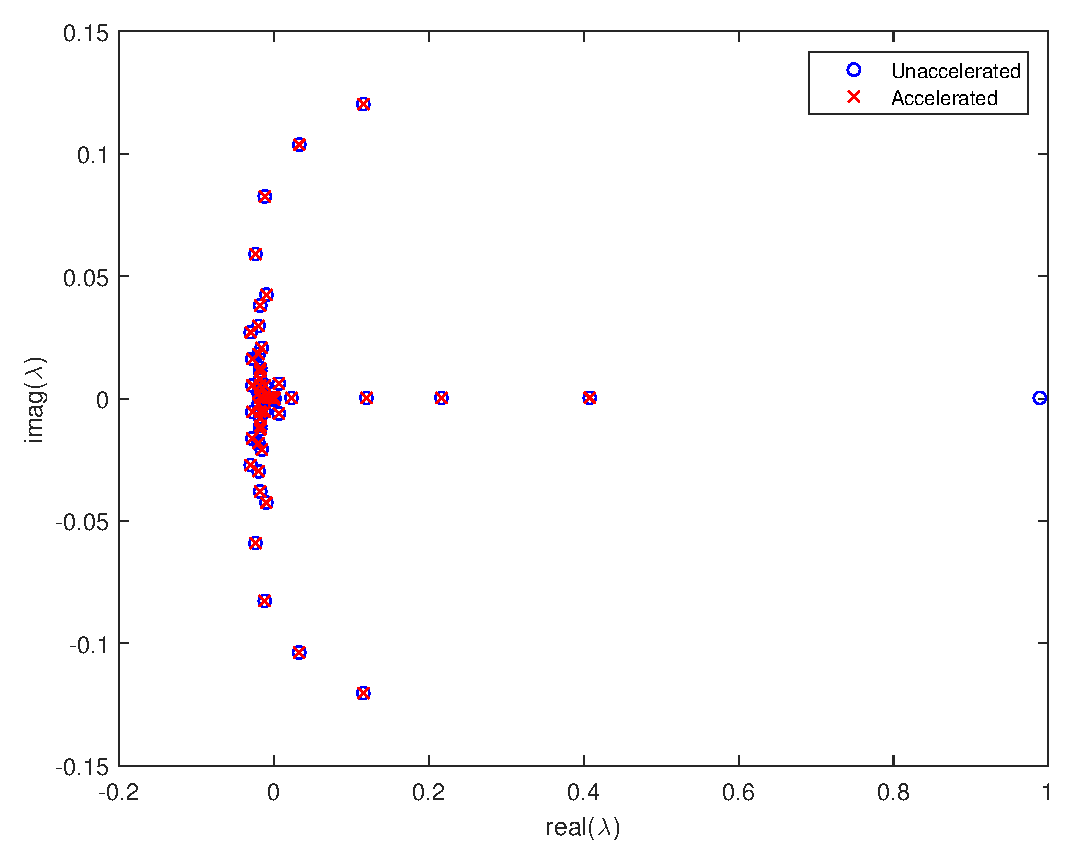
\includegraphics[width=0.75\textwidth]{images/IM1_Graph_FA_TG.eps}
}
\only<2>
{
\frametitle{\small Graphite Modified Two-Grid Flat Mode Eigenvalues}
\hspace*{1.1cm}
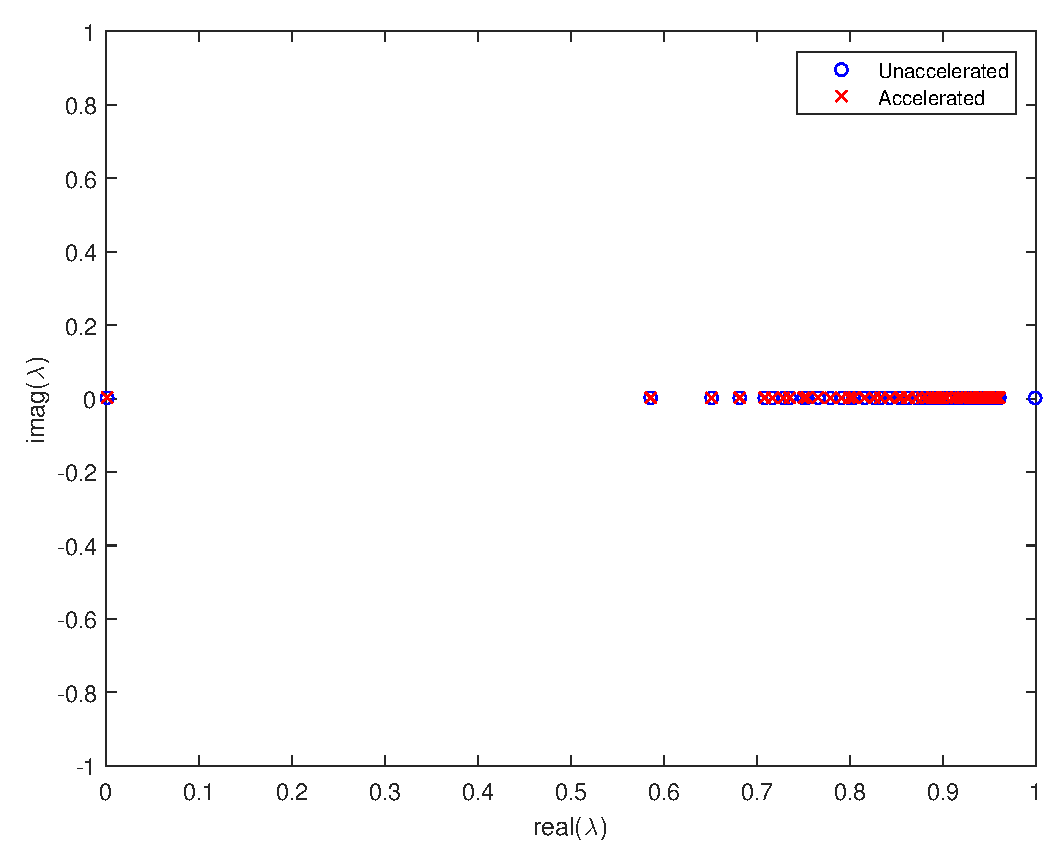
\includegraphics[width=0.75\textwidth]{images/IM1_Graph_FA_MTG.eps}
}
\only<3>
{
\frametitle{\small Graphite Multigroup Jacobi Acceleration Flat Mode Eigenvalues}
\hspace*{1.1cm}
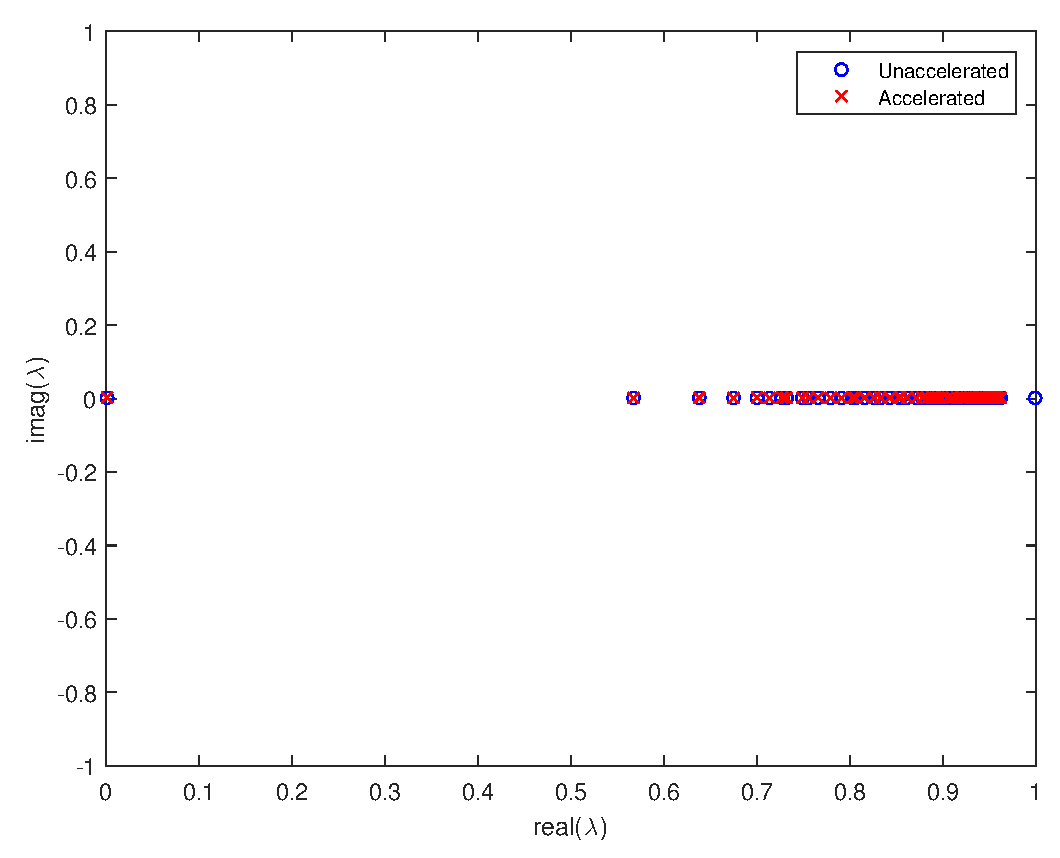
\includegraphics[width=0.75\textwidth]{images/IM1_Graph_FA_MJA.eps}
}
\only<4>
{
\frametitle{\small Graphite Multigroup Jacobi with Inner Acceleration Flat Mode Eigenvalues}
\hspace*{1.1cm}
\includegraphics[width=0.75\textwidth]{images/IM1_Graph_FA_MJIA.eps}
}
\end{frame}
% --------------------------------------------
\begin{frame}[t]\frametitle{2D Variant Results}{\footnotesize
\only<1>
{
\hspace*{1.75cm}
{}\includegraphics[width=0.60\textwidth]{images/2D_IM1_Variant_Layout.png}
}
\only<2>
{
\begin{block}{Two-Grid Results - $10^{-7}$ inner tolerance}
\begin{table}
\begin{tabular}{|c|c|c|c|c|}
\hline
Problem & Outer Iter. & Inner Iter. & 1-Group Sweeps & Solve Time (min)  \\
\hline \hline
\tcr{SI} & \tcr{361} & \tcr{185,422} &\tcr{185,422}  &  \tcr{486.50} \\ \hline
SI+DSA & 55 & 35,699 & 35,699 &  96.48 \\ \hline
GMRES & 38 & 41,575 & 41,575 &  128.63 \\ \hline
GMRES+DSA & 14 & 19,053 & 19,053  & 57.92  \\ \hline
\end{tabular}
\end{table}
\end{block}
\vspace{-3mm}
\begin{block}{Modified Two-Grid Results}
\begin{table}
\begin{tabular}{|c|c|c|c|c|}
\hline
Problem & Outer Iter. & Inner Iter. & 1-Group Sweeps & Solve Time (min)  \\
\hline \hline
\tcr{SI} & \tcr{536} & \tcr{77,632} & \tcr{77,632} & \tcr{275.83}  \\ \hline
SI+DSA & 73 & 10,846 & 10,846 &  40.60 \\ \hline
GMRES & 78 & 4,845 & 4,845 &  25.82 \\ \hline
GMRES+DSA & 26 & 1,881 & 1,881 & 11.09  \\ \hline
\end{tabular}
\end{table}
\end{block}
\vspace{-3mm}
\begin{block}{Multigroup Richardson Results}
\begin{table}
\begin{tabular}{|c|c|c|c|c|}
\hline
Problem & Outer Iter. & Inner Iter. & 1-Group Sweeps & Solve Time (min)  \\
\hline \hline
\tcr{SI} & \tcr{1} & \tcr{1,734} & \tcr{98,838} &  \tcr{111.07} \\ \hline
SI+DSA & 1 & 157 & 8,949 &  15.49 \\ \hline
GMRES & 1 & 118 & 6,726 &  8.65 \\ \hline
\tcb{GMRES+DSA} &  \tcb{1}& \tcb{35} & \tcb{1,995} &  \tcb{4.16} \\ \hline
\end{tabular}
\end{table}
\end{block}
}
}
\end{frame}
% --------------------------------------------
\begin{frame}[t]\frametitle{3D IM1 Results}{\footnotesize
\vspace{-2mm}
\begin{block}{Two-Grid Results}
\begin{table}
\begin{tabular}{|c|c|c|c|}
\hline
Problem & Outer Iter.  & 1-Group Sweeps & Solve Time (hr)  \\
\hline \hline
SI & - & -  & -  \\ \hline
SI+DSA & -  & - & -  \\ \hline
GMRES & -  & - & - \\ \hline
\tcr{GMRES+DSA} & \tcr{14} &  \tcr{11,104}  &  \tcr{$32.5^*$}  \\ \hline
\end{tabular}
\end{table}
\end{block}
\vspace{-2mm}
\begin{block}{Modified Two-Grid Results}
\begin{table}
\begin{tabular}{|c|c|c|c|}
\hline
Problem & Outer Iter.  & 1-Group Sweeps & Solve Time (hr)  \\
\hline \hline
SI & - &  - & -  \\ \hline
SI+DSA & -  & - & -  \\ \hline
\tcr{GMRES} & \tcr{81}  & \tcr{4,617 }& \tcr{$14.2^*$} \\ \hline
GMRES+DSA & 34 &  1,938  &  4.82  \\ \hline
\end{tabular}
\end{table}
\end{block}
\vspace{-2mm}
\begin{block}{Multigroup Richardson Results}
\begin{table}
\begin{tabular}{|c|c|c|c|}
\hline
Problem & Outer Iter. & 1-Group Sweeps & Solve Time (hr)  \\
\hline \hline
SI &  - & - & -  \\ \hline
SI+DSA & 256 &  14,592 & 11.2 \\ \hline
\tcm{GMRES} & \tcm{120} & \tcm{6,840} & \tcm{4.93} \\ \hline
\tcb{GMRES+DSA} & \tcb{31}& \tcb{1,767} & \tcb{1.76} \\ \hline
\end{tabular}
\end{table}
\end{block}
}
\end{frame}
% --------------------------------------------
%%%%%%%%%%%%%%%%%%%%%%%%%%%%%%%%%%%%%%%%%%%%%%%%%%%%%%%%%%%%%%%%%%%%%%%%%%%%%%%%%%%%%%%%%%%%%%
%%%%%%%%%%%%%%%%%%%%%%%%%%%%%%%%%%%%%%%%%%%%%%%%%%%%%%%%%%%%%%%%%%%%%%%%%%%%%%%%%%%%%%%%%%%%%%
\typeout{***********************************************************************************}
\typeout{Conclusions}
%%%%%%%%%%%%%%%%%%%%%%%%%%%%%%%%%%%%%%%%%%%%%%%%%%%%%%%%%%%%%%%%%%%%%%%%%%%%%%%%%%%%%%%%%%%%%%
% CONCLUSIONS SECTION
\section{Conclusions and Open Items}
\subsection{}
% --------------------------------------------
\begin{frame}[t]\frametitle{Conclusions}
\begin{block}{POLYFEM Conclusions}
\begin{enumerate}
\item
\item
\item
\item
\end{enumerate}
\end{block}
\begin{block}{DSA Conclusions}
\begin{enumerate}
\item
\item
\item
\item
\end{enumerate}
\end{block}
\end{frame}
% --------------------------------------------
\begin{frame}[t]\frametitle{Open Items}
\begin{block}{POLYFEM Open Items}
\begin{enumerate}
\item Quadratic serendipity basis functions on 3D polyhedra
\item Higher-order 2D serendipigy polygonal basis functions
\item Alternative integration schemes on polygons
\end{enumerate}
\end{block}
\begin{block}{DSA Open Items}
\begin{enumerate}
\item Mixed-mode parallelism with DSA preconditioning
\end{enumerate}
\end{block}
\end{frame}
% --------------------------------------------

%%%%%%%%%%%%%%%%%%%%%%%%%%%%%%%%%%%%%%%%%%%%%%%%%%%%%%%%%%%%%%%%%%%%%%%%%%%%%%%%%%%%%%%%%%%%%
\typeout{***********************************************************************************}
\typeout{We have reached the end}

\begin{frame}[plain]
   \frametitle{Thank you!}

\vspace{25mm}

\begin{columns}[b]

\column{0.7\textwidth}

\centering

{\Large Questions?}

\vspace{9mm}
\footnotesize
A special acknowledgment to the Department of Energy Rickover Fellowship Program in Nuclear Engineering, which provides strong support to its fellows and their professional development.

\end{columns}

\vspace{10mm}

\begin{columns}[b]

\column{0.5\textwidth}
\centering
{}\includegraphics[width=0.35\figwidth]{images/DOE_logo.png}\\

\column{0.5\textwidth}
\centering
{}\includegraphics[width=0.70\figwidth]{images/tamu_engineering.png}\\

\end{columns}

\end{frame}

%%%%%%%%%%%%%%%%%%%%%%%%%%%%%%%%%%%%%%%%%%%%%%%%%%%%%%%%%%%%%%%%%%%%%%%%%%%%%%%%%%%%%%%%%%%

\backupbegin
\appendix

%%%%%%%%%%%%%%%%%%%%%%%%%%%%%%%%%%%%%%%%%%%%%%%%%%%%%%%%%%%%%%%%%%%%%%%%%%%%%%%%%%%%%%%%%%%%
%%%%%%%%%%%%%%%%%%%%%%%%%%%%%%%%%%%%%%%%%%%%%%%%%%%%%%%%%%%%%%%%%%%%%%%%%%%%%%%%%%%%%%%%%%%%
\typeout{***********************************************************************************}
\typeout{Backup Slides}
\section{Backup Slides}
%%%%%%%%%%%%%%%%%%%
\subsection{Additional POLYFEM Results}
% --------------------------------------------

% --------------------------------------------
%%%%%%%%%%%%%%%%%%%
\subsection{Additional MIP Slides}
%%%%%%%%%%%%%%%%%%%
% --------------------------------------------

% --------------------------------------------
\backupend

\end{document}

